
%----------------------------------------------------------------------------------------
%	PACKAGES AND DOCUMENT CONFIGURATIONS
%----------------------------------------------------------------------------------------

\documentclass[12pt,a4paper]{article}

\usepackage[version=3]{mhchem} % Package for chemical equation typesetting
\usepackage{siunitx} % Provides the \SI{}{} and \si{} command for typesetting SI units
\usepackage{graphicx} % Required for the inclusion of images
\usepackage{natbib} % Required to change bibliography style to APA
\usepackage{amsmath} % Required for some math elements 
\usepackage{geometry}
\usepackage{enumerate}
\usepackage{textcomp}
\usepackage{siunitx}
\usepackage{hhline}
\usepackage{caption}
\usepackage{booktabs}
\usepackage{multirow}
\usepackage{float}
\usepackage{longtable}

\renewcommand{\labelenumi}{\alph{enumi}.} % Make numbering in the enumerate environment by letter rather than number (e.g. section 6)
\geometry{left=2.0cm,right=2.0cm,top=2.7cm,bottom=2.7cm}

%\usepackage{times} % Uncomment to use the Times New Roman font

%----------------------------------------------------------------------------------------
%	DOCUMENT INFORMATION
%----------------------------------------------------------------------------------------


\begin{document}
\thispagestyle{empty}
\begin{center}

\Large{ \textsc{\newline\rule{14.3cm}{0.05em}\newline\\UM-SJTU Joint Institute\\Physics Laboratory\\(Vp241)\\}}
\rule{14.3cm}{0.05em}
\LARGE{\textsc{\newline\newline\newline\newline\newline\\
Laboratory Report\\}}
\Large{\textsc{  \\ Exercise 5  \\ RC, RL, and RLC Circuits
} }

\end{center}

\begin{description}
    \item[] 
    \item[] 
    \item[] 
    \item[] 
    \item[] 
    \item[]
    \item[]
    \item[]
    \item[]\qquad \qquad Name: Zhang Yifei \qquad ID:519370910103   \qquad    Group:10
    \item[]\qquad \qquad Date: \today
\end{description}

\newpage
\setcounter{page}{1}
\section{Abstract}
\qquad In this experiment, different characteristics of RC,RL and RLC circuits are studied and proved. We basically studied the time constant, different regimes and their waveforms, and the reasonance circuit. Calculations, figures and plots are all used to better illustrate the result. Also, we discuss the uncertainty and possible error in this experiment.


\section{Introduction}
\subsection{Motivation}
\qquad This experiment helps us better understand the RC, RL, and RLC circuits and also the characteristics of them, including the phase-frequency and their phenomenon. Also, this experiment helps us know better about the real circuit and the use of signal generator.
\subsection{Theoretical Background}

\subsubsection{Transient Processes in RC, RL, RLC Series Circuits}

\quad \textbf{RC Series Circuits}\par
In a RC circuit, the process of charging or discharging of the capacitor is an one
of the transient process. For first half of the cycle, the square-wave voltage is $U(t) = \mathcal{E}$ . 
\begin{figure}[h]
	\centering
	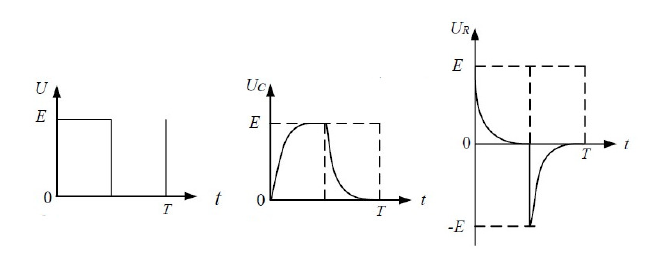
\includegraphics[width=14cm]{1}
	\caption{Charging/discharging curves for a RC series circuit.}
	\label{fig:front}
\end{figure}
\par For the second half-cycle, the square-wave voltage is zero,and the capacitor discharges through the resistor. The loop equation for the charging process is
$$RC\frac{dU_c}{dt}+U_C=\mathcal{E}$$
\par And we can get
$$U_R=iR=-\mathcal{E} e^{-\frac{t}{RC}}$$
\par where the magnitudes of both $U_C$ and $U_R$ decrease exponentially with time. And $RC = \tau$ is called the time constant of the circuit, and characterizes the
dynamics of the transient process. \par Another characteristics related to the time
constant is the half-life period $T_{1/2}$, which indicates the time needed for $U_C$ to decrease to a half of the initial value (or
increase to a half of the terminal value), and may be also used to characterize the dynamics of the transient process. And the quantities are related by the equation $$T_{1/2}=\tau \ln{2}\approx 0.693\tau.$$

\textbf{RL Series Circuits}\par
Similarly, we obtain 
$$\tau=L/R ~~and~~ T_{1/2}=L\ln{2}/R$$


\textbf{RLC Series Circuit}\par 

Similarly we obtain
$$\frac{d^2U_c}{dt^2}+2\beta\frac{dU_C}{dt}+\omega_0^2U_C=\omega_0^2\mathcal{E}$$\par
where $\beta=R/2L$ and $\omega_0=1/\sqrt{LC}$.\par

\begin{itemize}
    \item  If $\beta^{2}-\omega_{0}^{2}<0$ (weak damping), the system is in the underdamped regime and the solution to the initial value problem is of the form
    $$
    U_{C}=\mathcal{E}-\mathcal{E} e^{-\beta t}\left(\cos \omega t+\frac{\beta}{\omega} \sin \omega t\right)
    $$
    where $\omega=\sqrt{\omega_{0}^{2}-\beta^{2}}$
    \item  If $\beta^{2}-\omega_{0}^{2}>0$, the system is in the overdamped regime with the solution of the form
    $$
    U_{C}=\mathcal{E}-\frac{\mathcal{E}}{2 \gamma} e^{-\beta t}\left[(\beta+\gamma) e^{\gamma t}-(\beta-\gamma) e^{-\gamma t}\right]
    $$
    where $\gamma=\sqrt{\beta^{2}-\omega_{0}^{2}}$
    \item Finally, if $\beta^{2}-\omega_{0}^{2}=0,$ the system is said to be critically damped, and
    $$
    U_{C}=\mathcal{E}-\mathcal{E}(1+\beta t) e^{-\beta t}
    $$
\end{itemize}

\begin{figure}[h]
	\centering
	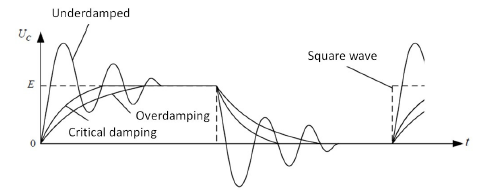
\includegraphics[width=11cm]{2}
	\caption{Three different regimes of transient processes in a RLC series circuit.}
	\label{fig:front}
\end{figure}

\subsubsection{RC, RL Steady–State Circuits}
\quad When a sinusoidal alternating input voltage is provided to a $R C$ (or $R L$ ) series circuit, the amplitude and the phase of the voltage will change with the frequency. 
$$
\varphi=\tan ^{-1}\left(\frac{U_{L}}{U_{R}}\right)=\tan ^{-1}\left(\frac{\omega L}{R}\right), \quad \varphi=\tan ^{-1}\left(-\frac{U_{C}}{U_{R}}\right)=\tan ^{-1}\left(-\frac{1}{\omega R C}\right)
$$

\subsubsection{RLC Resonant Circuit}
\quad \textbf{RLC Series Circuit}\par
A generic RLC series circuit is shown in Figure 3. 
\begin{figure}[H]
	\centering
	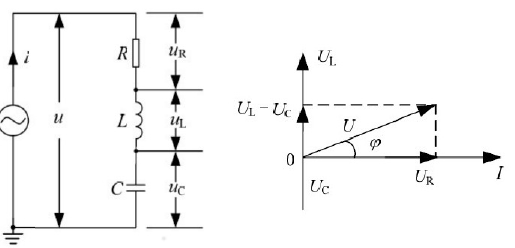
\includegraphics[width=11cm]{3}
	\caption{RLC series circuit.}
	\label{fig:front}
\end{figure}
\par The phase difference between the current and the voltage in the circuit
$$
\varphi=\tan ^{-1}\left(\frac{U_{L}-U_{C}}{U_{R}}\right)=\tan ^{-1}\left(\frac{\omega L-\frac{1}{\omega C}}{R}\right)
$$

\textbf{Resonance}\par
If the frequency of the input signal provided by the source satisfies the condition
$$
\omega_{0} L=\frac{1}{\omega_{0} C}, \quad \text { or, equivalently } ~~\omega_{0}=\frac{1}{\sqrt{L C}}
$$
\par the total impedance will reach a minimum, $Z_{0}=R$. Note that the resistance $R$ in a real circuit includes the internal resistance and all kinds of alternating-current power losses, so its actual value will be greater than the theoretical one.

When the current reaches its maximum, $I_{\mathrm{m}}=U / R,$ the circuit is said to be at resonance. The frequency at which the resonance phenomenon occurs, is called the resonance frequency. 
$$
f_{0}=\frac{\omega_{0}}{2 \pi}=\frac{1}{2 \pi \sqrt{L C}}
$$
 
\begin{figure}[H]
	\centering
	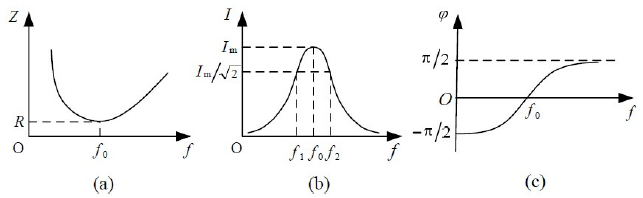
\includegraphics[width=13cm]{4}
	\caption{The impedance, the current and the phase difference as functions of the frequency for a RLC series circuit (generic sketches).}
	\label{fig:front}
\end{figure}

\textbf{Quality Factor}\par
For a circuit driven at the resonance frequency, the ratio of UL (or UC) to
U is called the quality factor Q of a resonant circuit$$Q=\frac{U_L}{U}={\omega_0L}{R}$$ \\

The quality factor can also be found as $$Q=\frac{f_0}{f_2-f_1}$$where f1 and f2 are two frequencies such that $I(f_1) = I(f_2) = I_m/\sqrt{2}$.
\par The equations and theories are all collected from books and manual, see reference 123
\section{Description of experiment}
\subsection{Apparatus}
\qquad The measurement setup consists of the following main elements: a signal generator, an
oscilloscope, a digital multimeter, a wiring board, a fixed resistor , a variable
resistor, a capacitor, as well as one inductor. And a collection of the uncertainty is shown in Table \ref{Apparatus Uncertainty}
\begin{table}[H]
    \centering
    \begin{tabular}{ccc}\hline
    {Quantity} & {Apparatus} & {Precision} \\\hline
    R                 & digital multimeter & 0.01{[}$\Omega ${]}         \\
    f                 & signal generator   & 0.001{[}Hz{]}        \\
    $\epsilon$                 & signal generator   & 0.001{[}$V_{pp}${]}        \\
    C                 & digital multimeter & 0.01{[}nF{]}         \\
     $T_{\frac{1}{2}}$                 & oscilloscope       & 0.01{[}$\mu s${]}        \\\hline
    \end{tabular}
    \caption{Apparatus Uncertainty}
    \label{Apparatus Uncertainty}
\end{table}
\subsection{Measurement Procedure}
\subsubsection{RC, RL Series Circuit}
\begin{enumerate}[1.]
    \item First we assemble a circuit with resistor and capacitor, connect the wave source and signal generator. Observe the change of the waveform when the time constant is smaller or greater than the period of the square–wave. Choose the frequency that allows the capacitor to fully charge/discharge.
    \item Measure the $T_{1/2}$, calculate the time constant and compare with the theoretical value.
    \item Change capacitor into inductor, repeat the above steps.
\end{enumerate}
\subsubsection{RLC Series Circuit}
\begin{enumerate}[1.]
    \item Use a capacitor, inductor and variable resistor to assemble a RLC series circuit. Observe the waveform when the capacitor voltage in the underdamped,
    critically damped, and overdamped regimes.
    \item Adjust the variable resistor to the critically damped regime. Find $T_{1/2}$ and get $\tau$, compare the theoretical value.
\end{enumerate}
\subsubsection{RLC Resonant Circuit}
\qquad Apply a sinusoidal input voltage $U_{\mathrm{i}}$ to the $R L C$ series circuit, change the frequency, then observe the change of the voltage $U_{R}$ for a fixed resistor $R,$ as well as the phase difference between $U_{R}$ and $U_{\mathrm{i}}$. Measure how $U_{R}$ changes with $U_{\mathrm{i}}$ and calculate the phase difference according to Figure $4 .$ Plot the graphs $I / I_{m}$ vs. $f / f_{0}$ and $\varphi$ vs. $f / f_{0} .$ Estimate the resonance frequency and calculate the quality factor $Q$.

\section{Results}
\subsection{Measurement of RC series circuit}
From the lab we captured a screen shot of the RC circuit. We see the charging/discharging ofthe capacitor from the curve. The parameters of the RC series circuit are shown in Table \ref{measurement data for RC series circuit.}.
\begin{figure}[H]
    \centering
    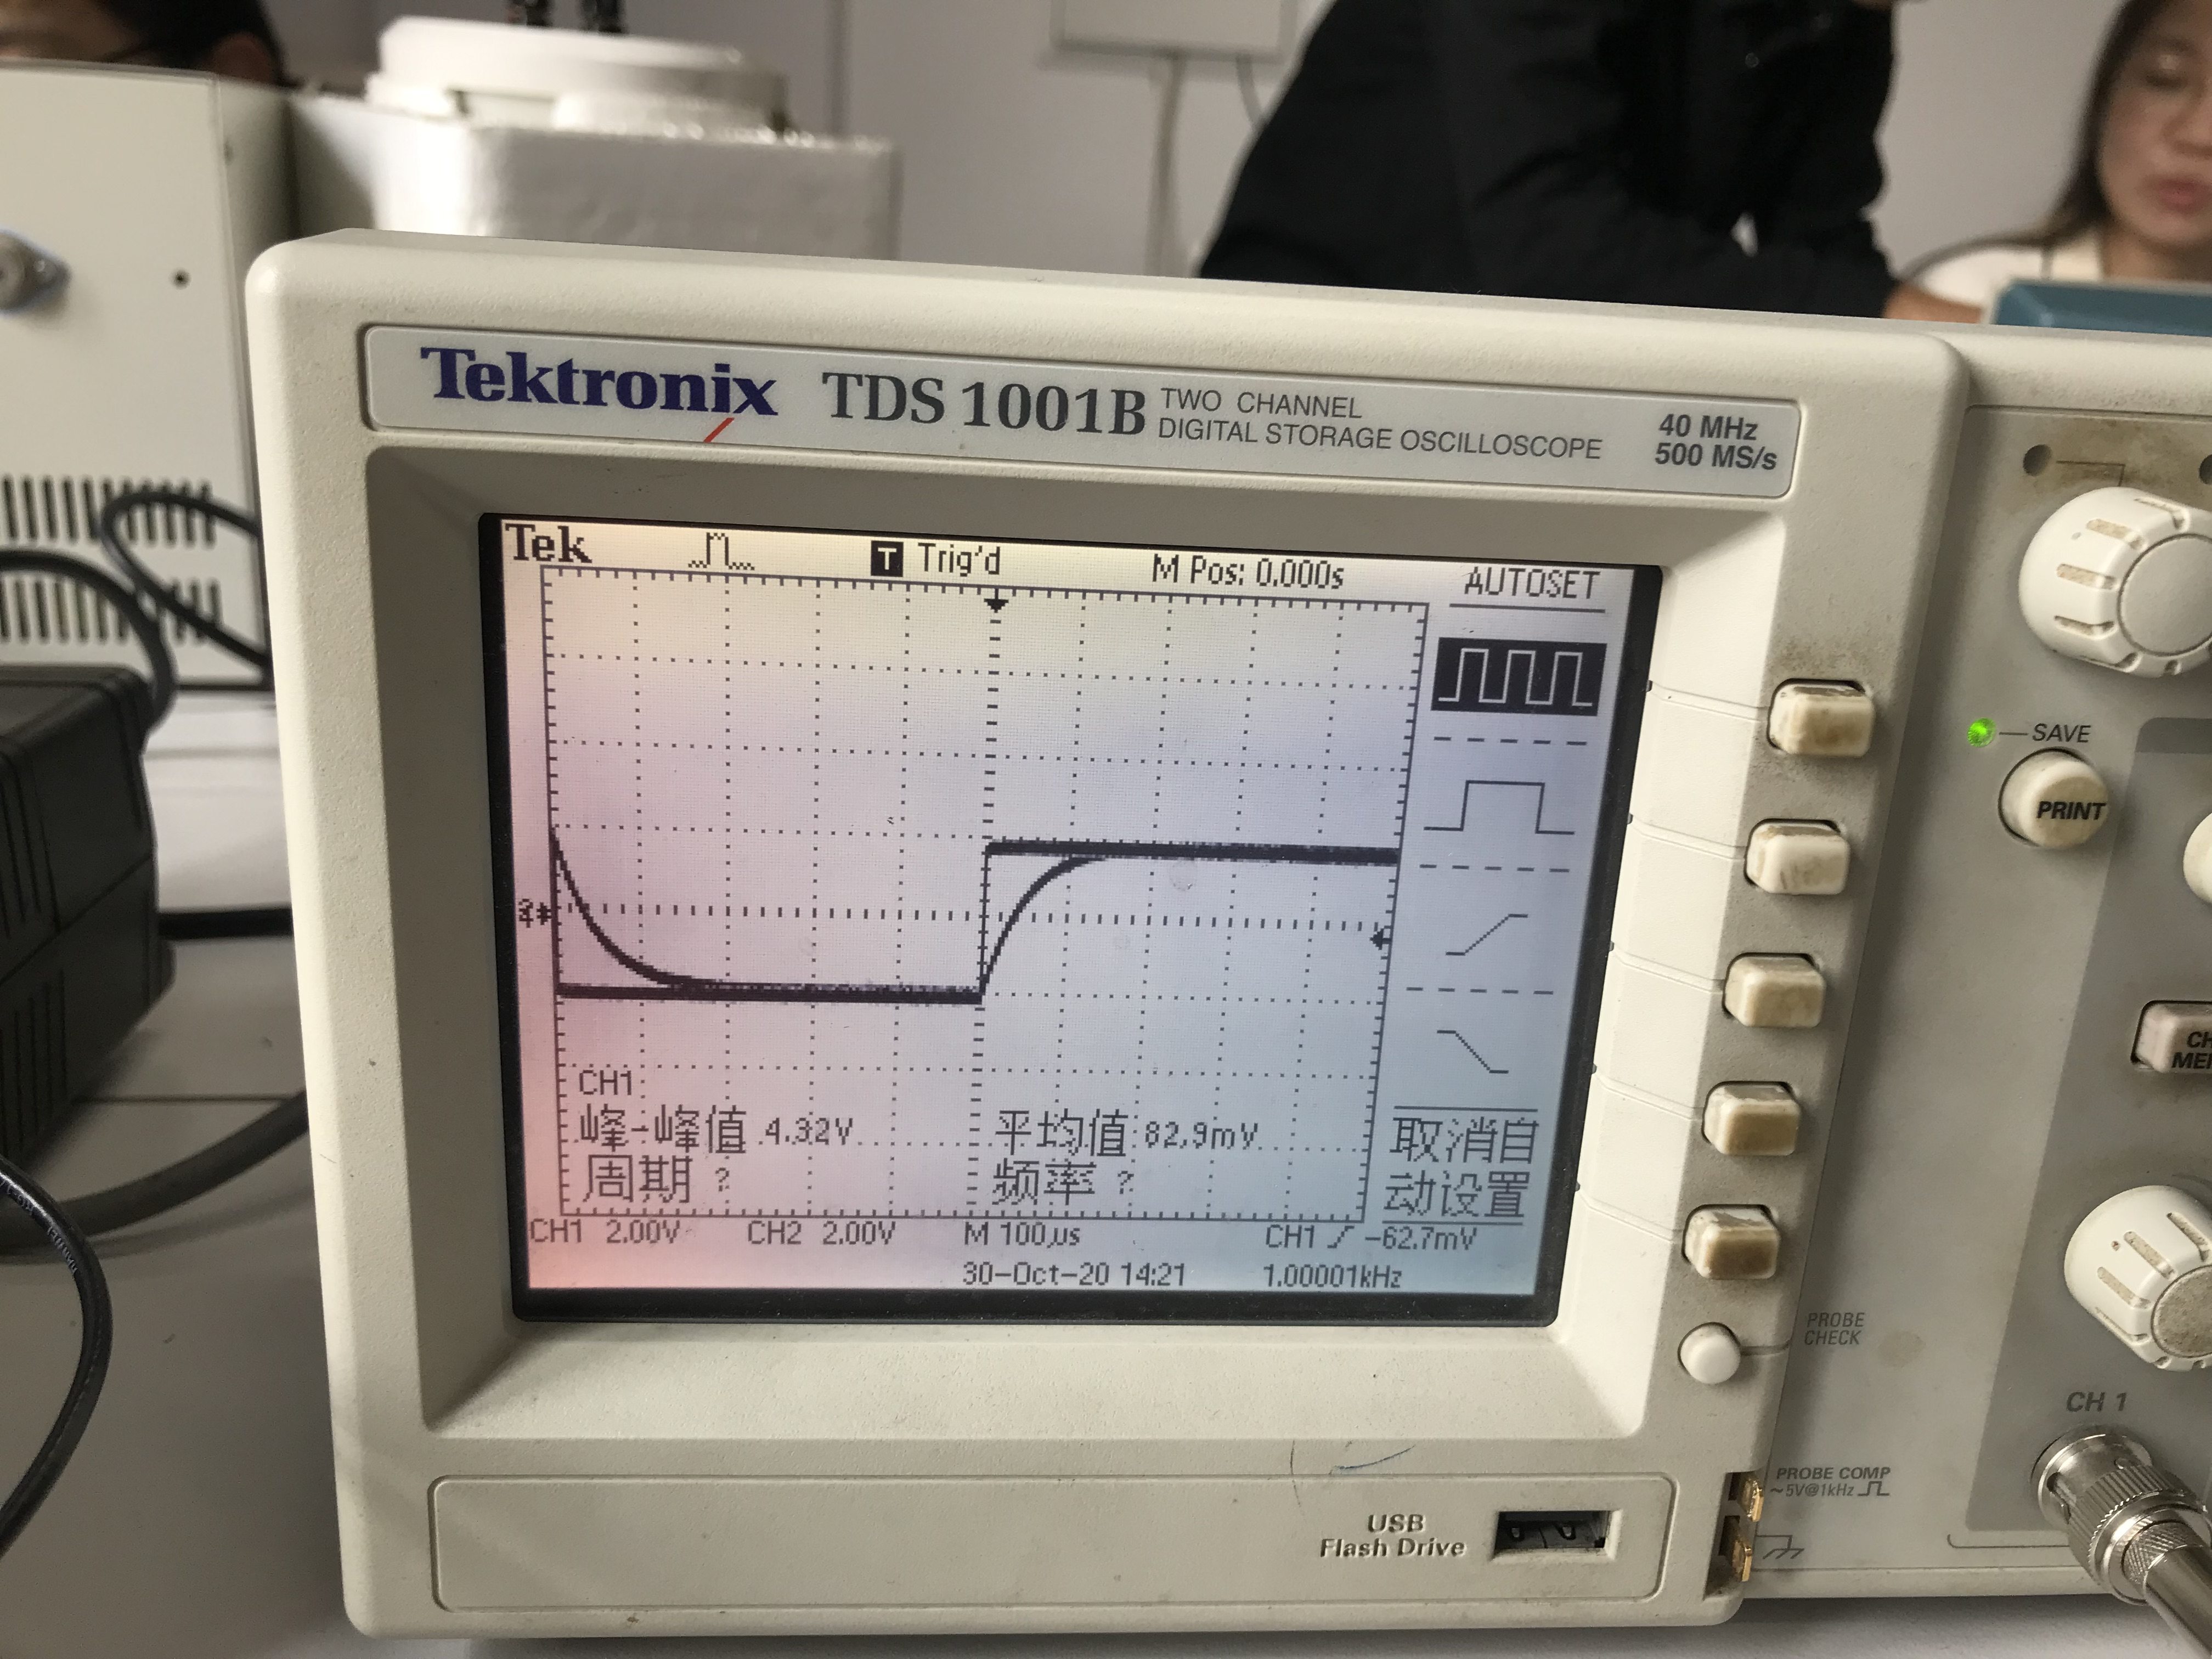
\includegraphics[scale=0.08]{p1.jpeg}
    \caption{Screen capture of RC circuit.}
    \label{Screen capture of RC circuit.}
\end{figure}
\begin{table}[H]
    \centering
    \begin{tabular}{ccccc}\hline
    R[$\Omega$]$\pm 0.01[\Omega]$     & f[kHz]$\pm 1\times 10^{-6}[kHz]$         &  $\epsilon[V]\pm 0.001[V]$     & C$[nF]\pm 0.01[nF]$      & T$[\mu s]\pm 0.01[\mu s]$     \\\hline
    99.94 & 1.000000 & 4.000 & 232.02 & 32.00\\\hline
    \end{tabular}
    \caption{$T_{1/2}$ measurement data for RC series circuit.}
    \label{measurement data for RC series circuit.}
\end{table}
\par We then have experimental and theoretical value to be:
$$\tau_{ex}=\frac{T_{1/2}}{ln2}=46.167\pm 0.014[\mu s]$$
$$\tau_{th}=RC=23.188\pm 0.003[\mu s]$$
\par The relative error is $99.1\%$.
\subsection{Measurement of RL Series Circuit.}
The parameters of the RC series circuit are shown in Table \ref{T1/2 measurement data for RL series circuit.}. From which we can calculate

\begin{table}[H]
    \centering
    \begin{tabular}{ccccc}
    \hline
    R{[}$\Omega${]}$\pm 0.01[\Omega]$ & f{[}kHz{]}$\pm 1\times 10^{-6}[kHz]$ & $\epsilon[V]\pm 0.001[V]$ & L$[H]$ & T$[\mu s]\pm 0.01[\mu s]$ \\ \hline
    99.94                             & 1.000000                             & 4.000                     & 0.01    & 72.00                     \\ \hline
    \end{tabular}
    \caption{$T_{1/2}$ measurement data for RL series circuit.}
    \label{T1/2 measurement data for RL series circuit.}
\end{table}
\begin{figure}[H]
    \centering
    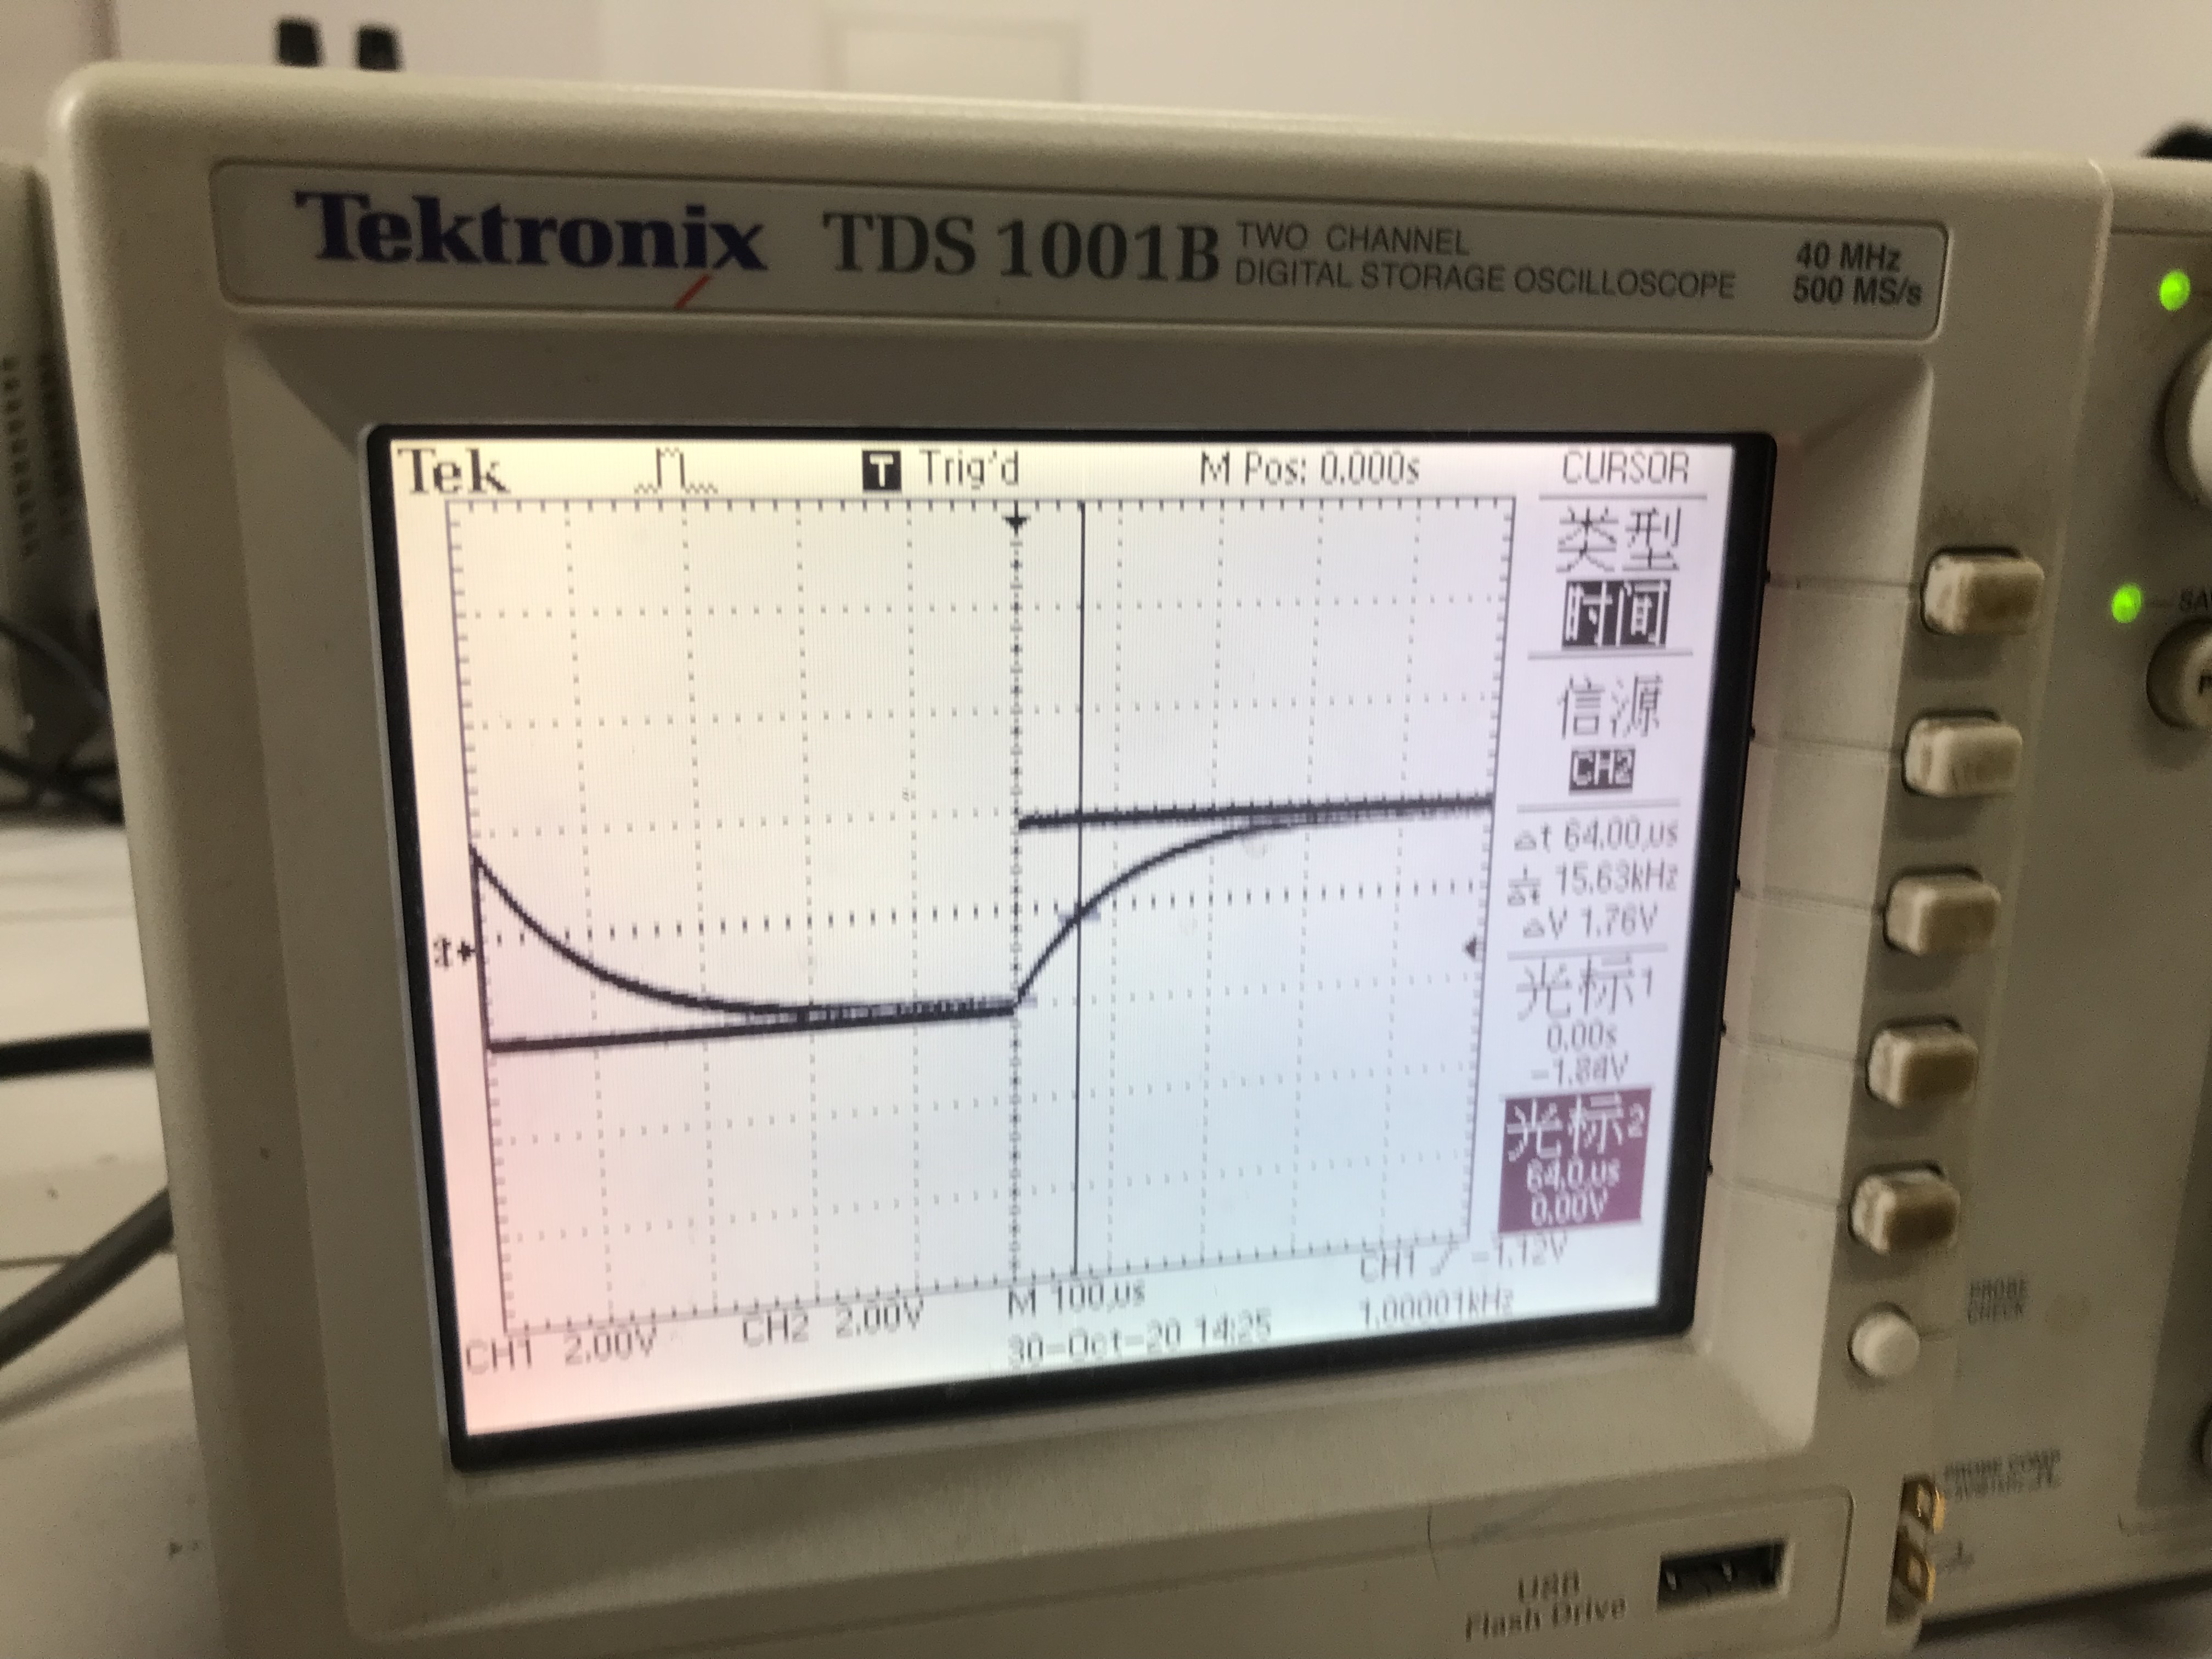
\includegraphics[scale=0.08]{p2.jpeg}
    \caption{Screen capture of RL circuit.}
    \label{Screen capture of RL circuit.}
\end{figure}
\par We then have experimental and theoretical value to be:
$$\tau_{ex}=\frac{T_{1/2}}{ln2}=103.874\pm 0.014[\mu s]$$
$$\tau_{th}=\frac{L}{R}=100.1\pm 1.0[\mu s]$$
\par The relative error is $3.8\%$.


\subsection{Measurement of RLC Series Circuit.}
\qquad In the lab we captured the wave shown on the oscillator under three damping situations.
\par Adjusting the resistance we also found the point where the critical damping occurs. The data
under critically-damped situation are recorded in Table \ref{T1/2 measurement data for critically damped RLC series circuit.}.
\begin{table}[H]
    \centering
    \begin{tabular}{cccccc}
    \hline
    R{[}$\Omega${]}$\pm 0.01[\Omega]$ & C$[nF]\pm 0.01[nF]$       & f{[}kHz{]}$\pm 1\times 10^{-6}[kHz]$ & $\epsilon[V]\pm 0.001[V]$ & L$[H]$ & T$[\mu s]\pm 0.01[\mu s]$ \\ \hline
    99.94                             & 233.02 & 1.000000                             & 4.000                     & 0.01    & 112.00                    \\ \hline
    \end{tabular}
    \caption{$T_{1/2}$ measurement data for critically damped RLC series circuit.}
    \label{T1/2 measurement data for critically damped RLC series circuit.}
\end{table}
And then we can calculate the theoretical and experimental value for $\tau$.
$$\tau_{ex}=\frac{T_{1/2}}{1.68}=66.667\pm 0.006[\mu s]$$
$$\tau_{th}=\sqrt{LC}=48.2721\pm 0.0010[\mu s]$$
The relative error is $38.1\%$.

\begin{figure}[H]
    \centering
    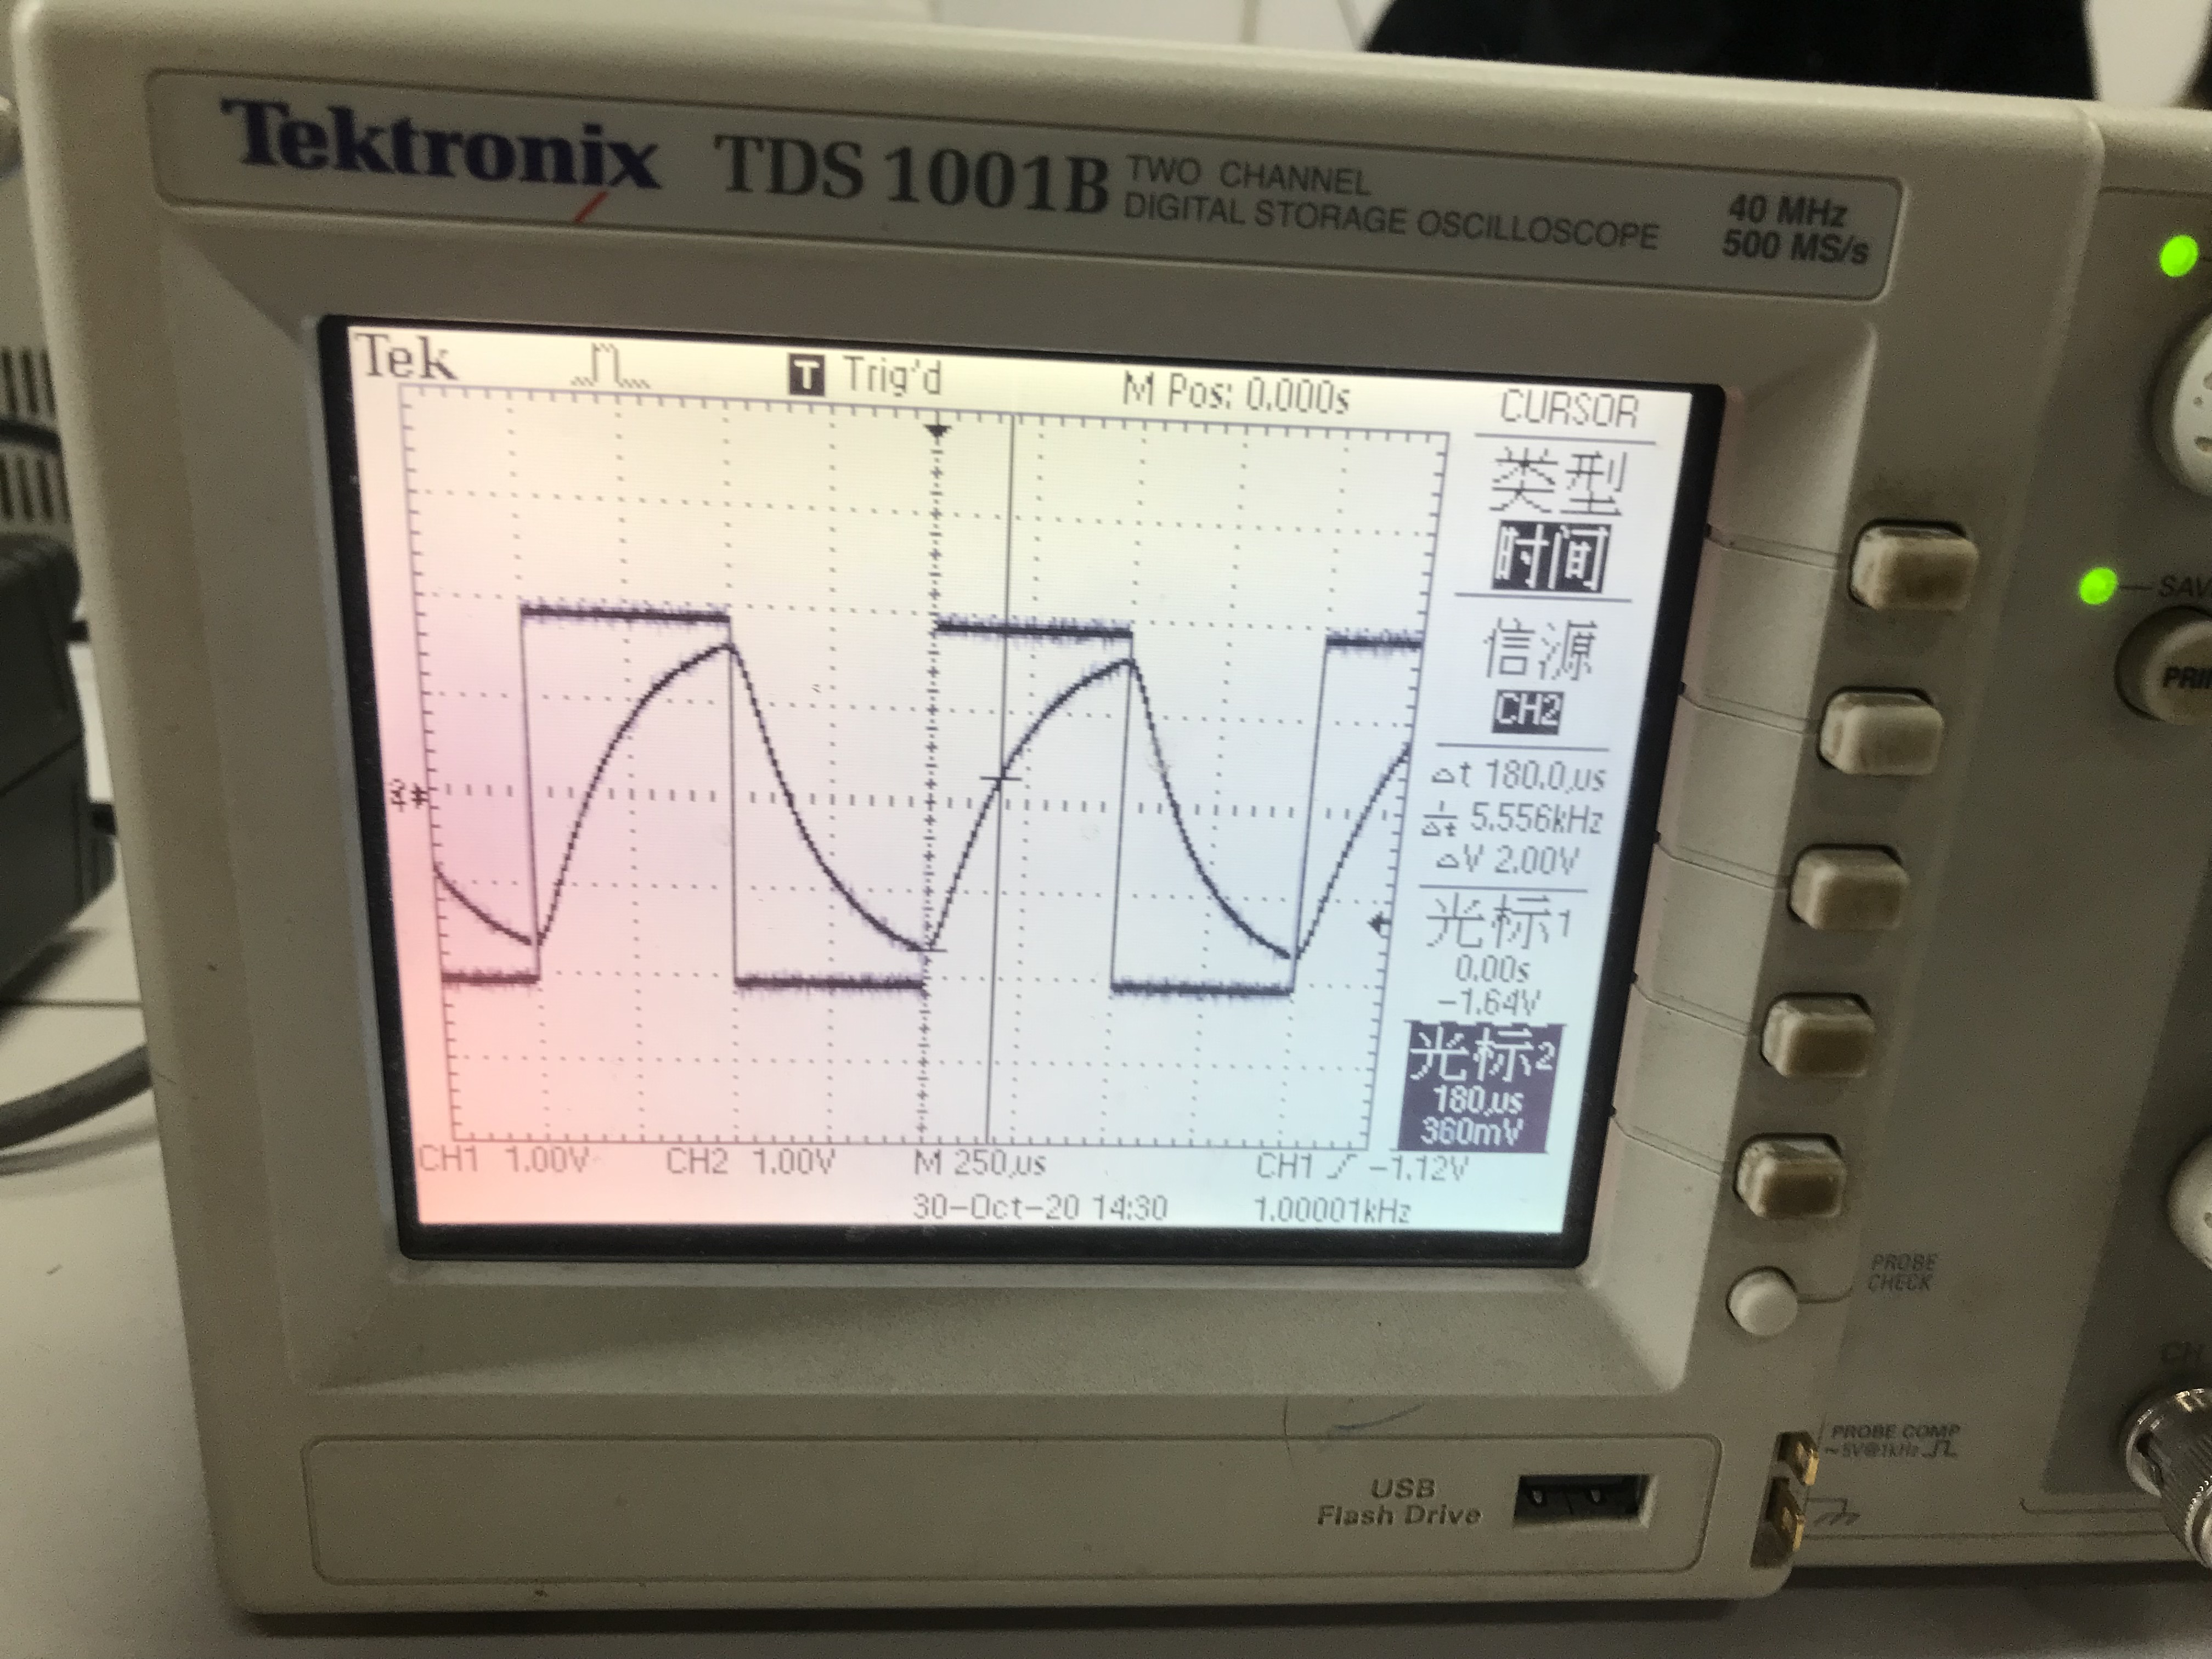
\includegraphics[scale=0.1]{over.jpeg}
    \caption{ Screen capture of over-damped situation.}
    \label{ Screen capture of over-damped situation.}
\end{figure}
\begin{figure}[H]
    \centering
    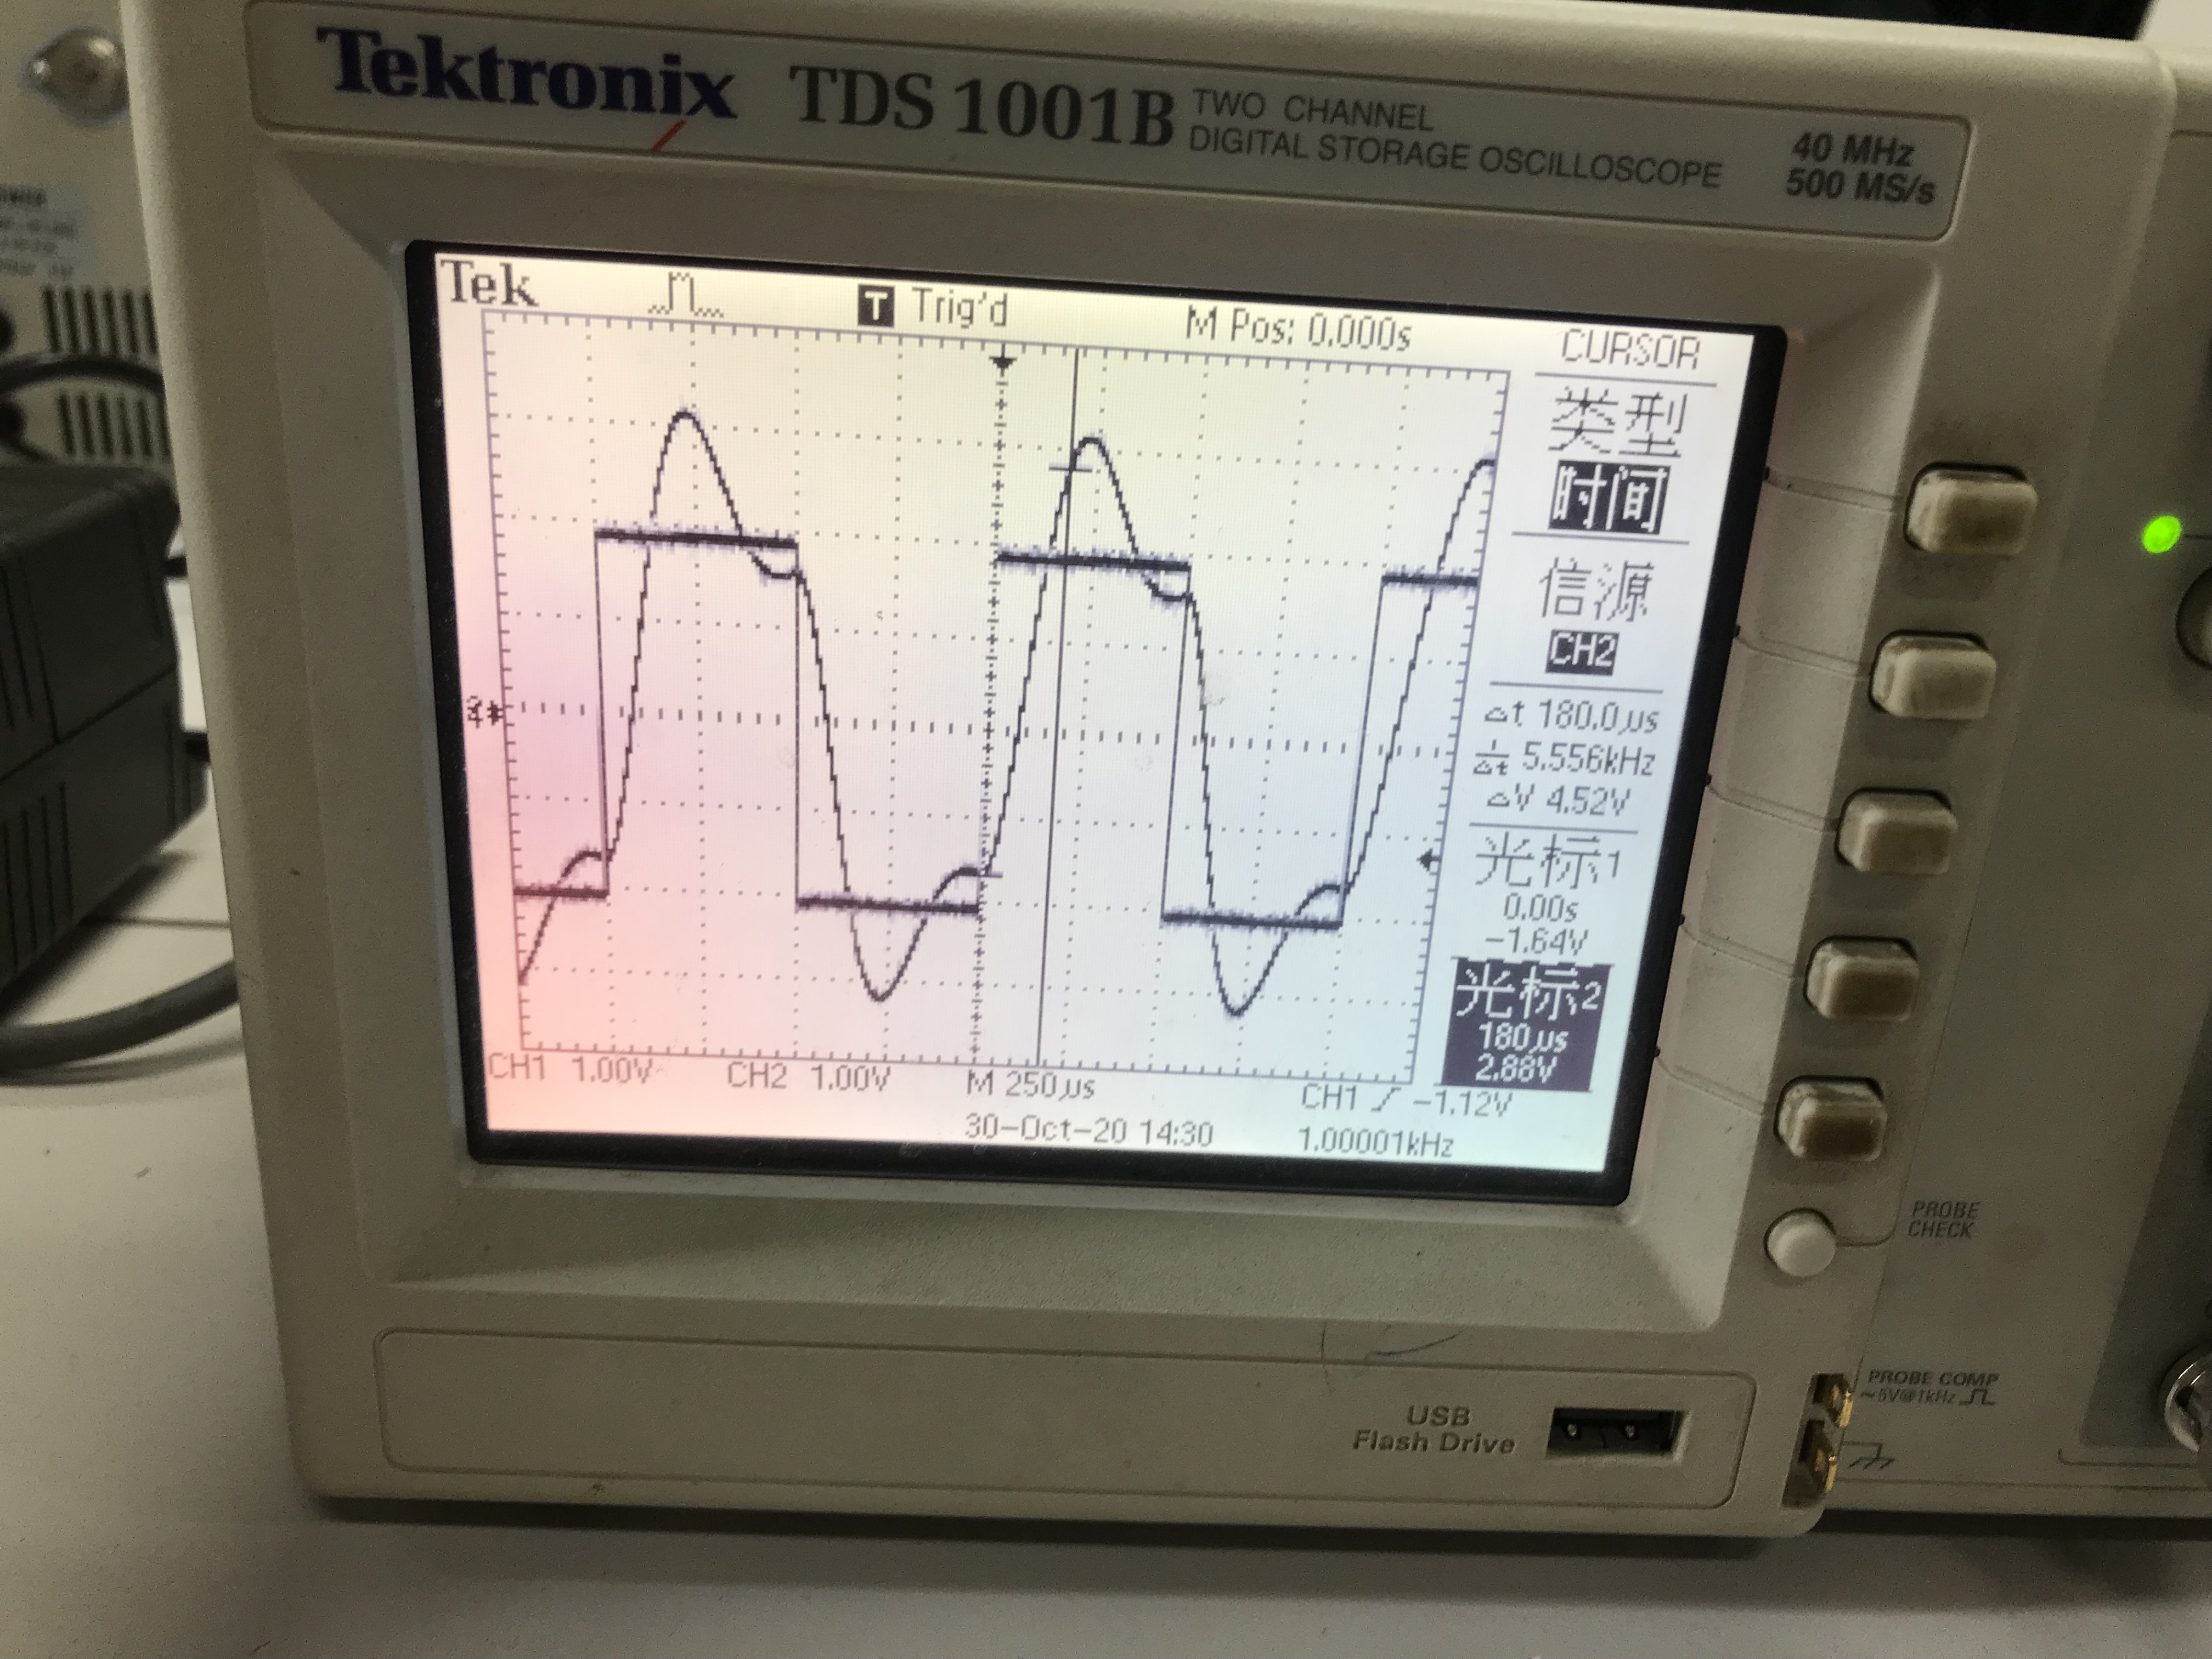
\includegraphics[scale=0.085]{under.jpeg}
    \caption{ Screen capture of under-damped situation.}
    \label{ Screen capture of under-damped situation.}
\end{figure}
\begin{figure}[H]
    \centering
    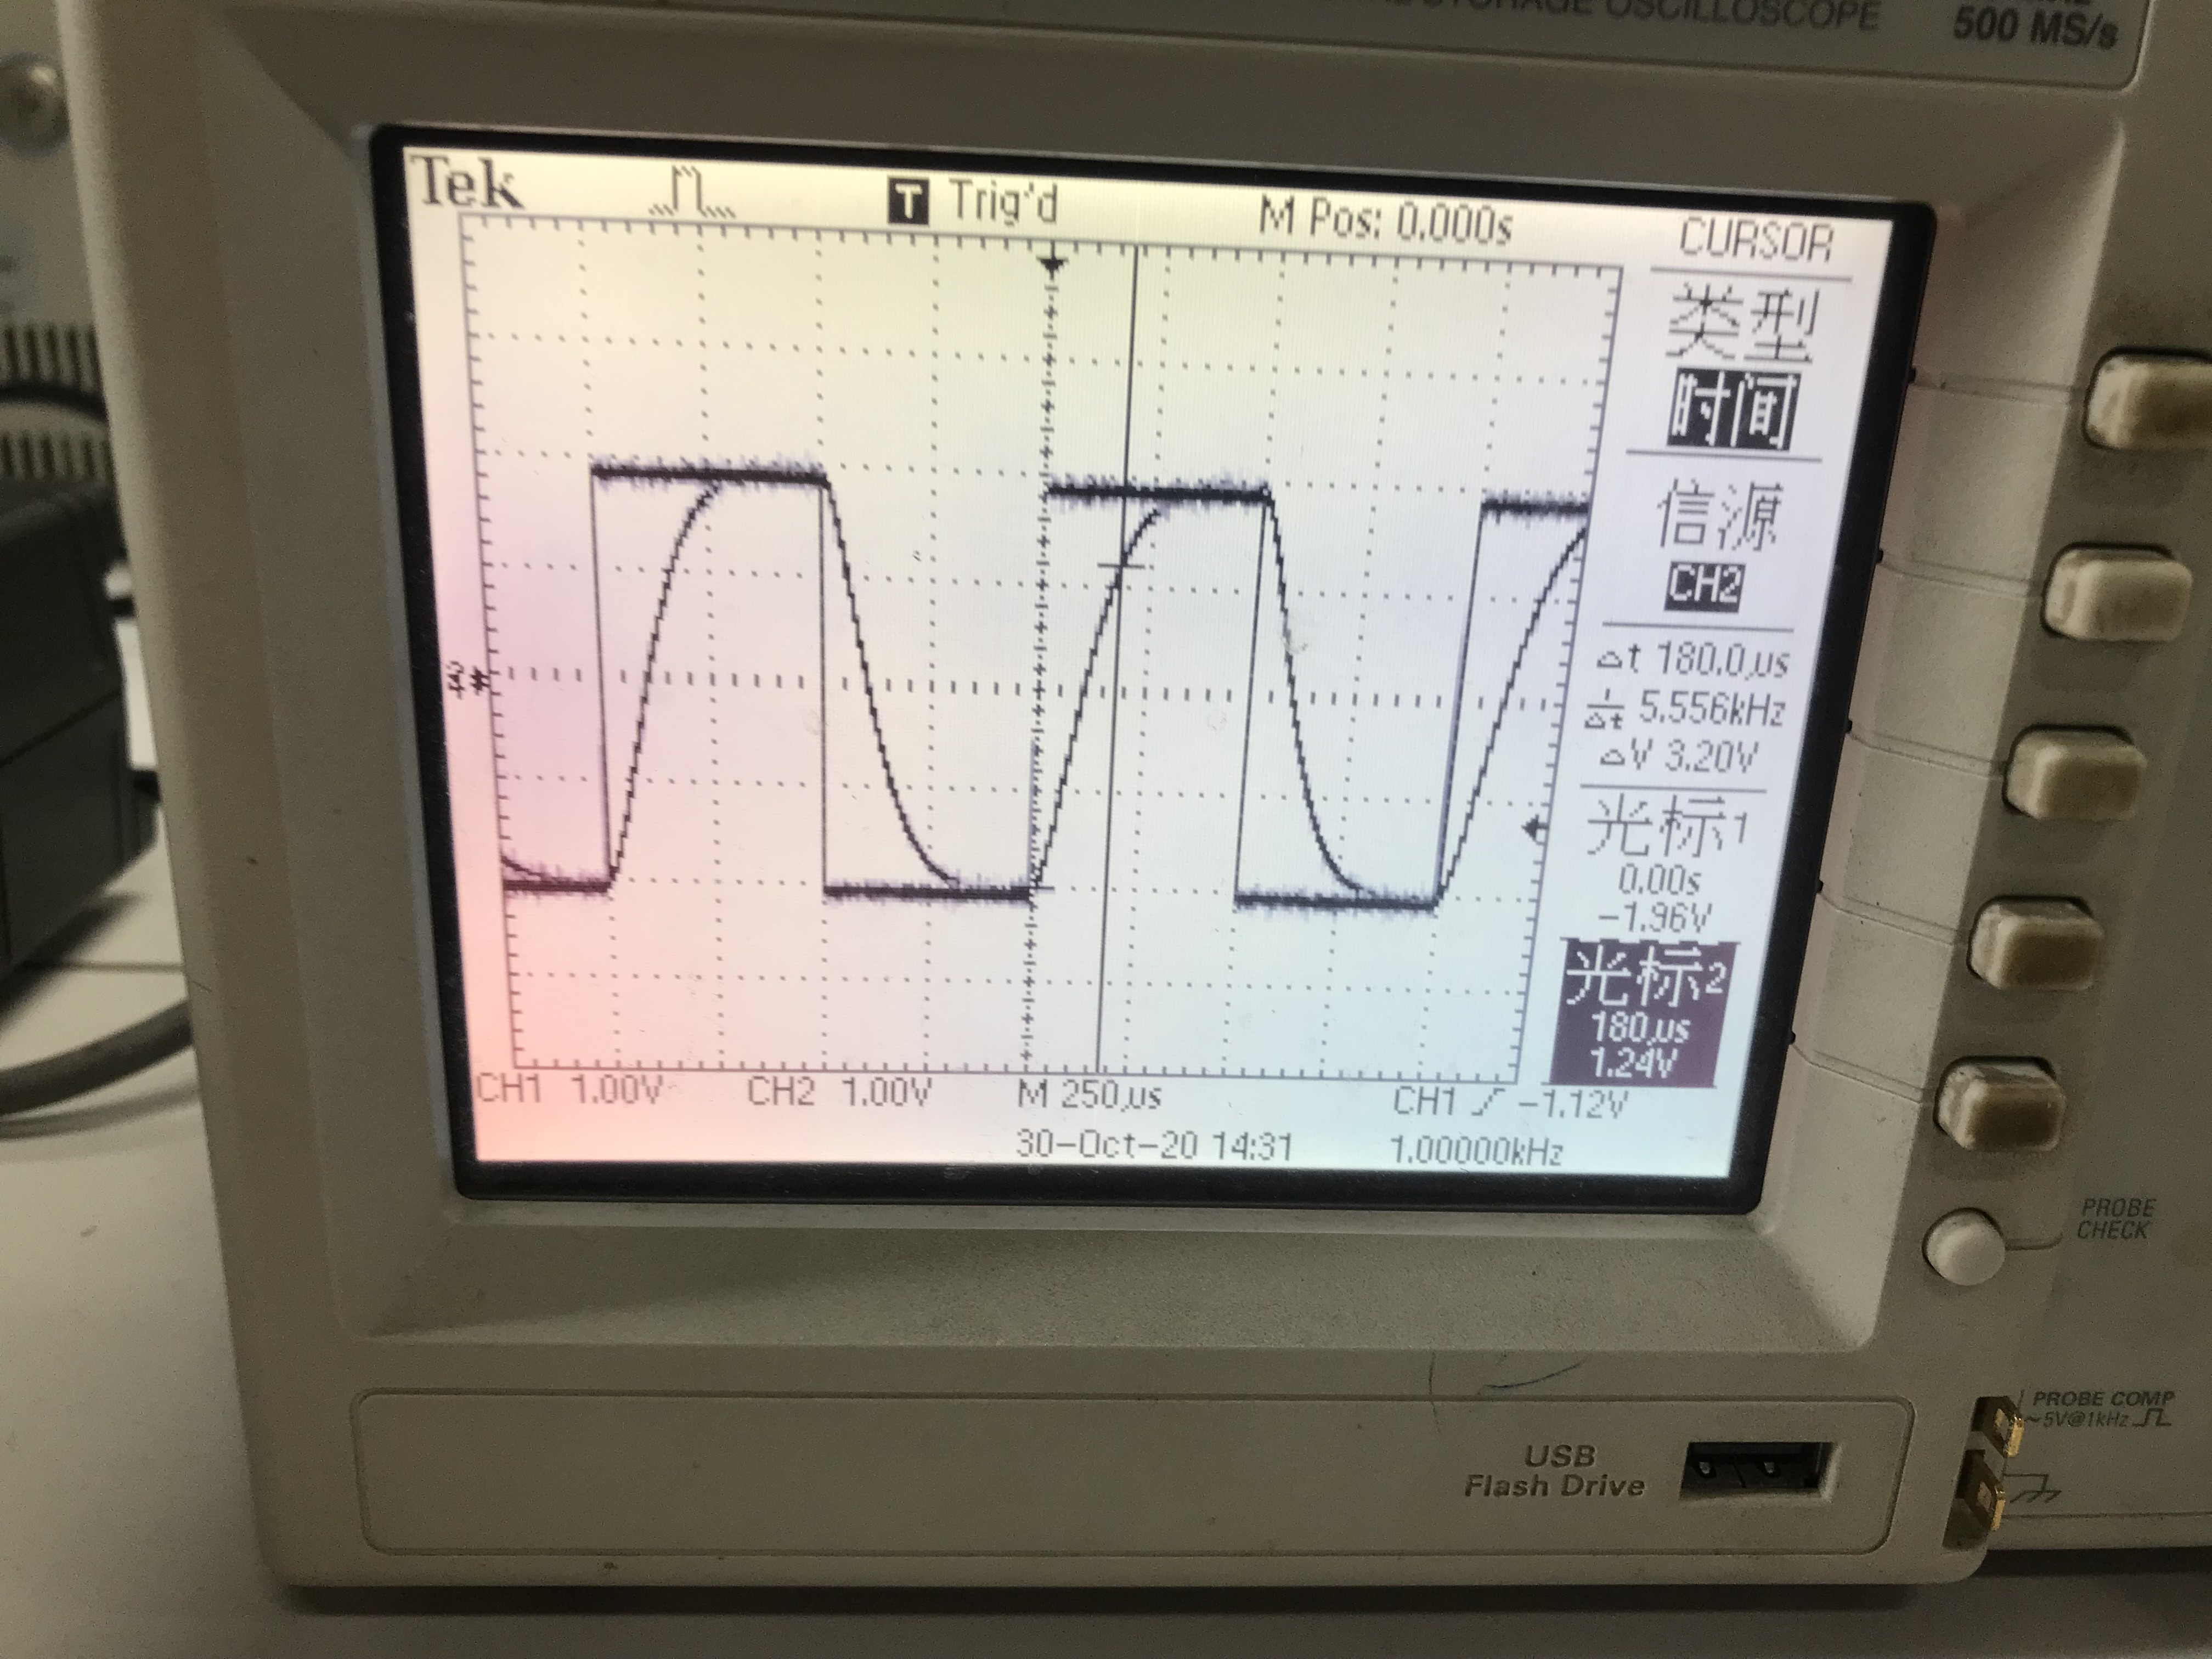
\includegraphics[scale=0.085]{critical.jpeg}
    \caption{ Screen capture of critical-damped situation.}
    \label{ Screen capture of critical-damped situation.}
\end{figure}
\subsection{Measurement of RLC Resonant Circuit.}
\qquad All related data is shown in Table . It's worth mentioning that the units for f is Hz, for v is V, for $\phi$ is rad, and for all relative parameters there are no unit. Changing the input frequency, we observe the change of $U_R$ for a fixed resistor R. The parameters are unchanged and the changing of $U_R$ is recorded in Table \ref{biggest}.



\begin{table}[H]
    \begin{tabular}{|c|c|c|c|c|c|c|c|c|c|}
    \hline
    \textbf{f} & \textbf{$U_R$} & \textbf{I/Im} & \textbf{$\mu$I/Im} & \textbf{f/f0} & \textbf{$\mu$f/f0} & \textbf{$\phi_{ex}$} & \textbf{$\mu\phi_{ex}$} & \textbf{$\phi_{theo}$} & \textbf{$\mu\phi_{theo}$} \\ \hline
    316.970        & 0.40           & 0.1042            & 0.0003                 & 0.1368000         & 0.0000004              & 1.4664                   & 0.0003                      & -1.524000                  & 0.000005                      \\ \hline
    476.060        & 0.64           & 0.1667            & 0.0003                 & 0.2054600         & 0.0000004              & 1.4033                   & 0.0003                      & -1.499800                  & 0.000007                      \\ \hline
    696.940        & 0.96           & 0.2500            & 0.0003                 & 0.3007900         & 0.0000005              & 1.3181                   & 0.0003                      & -1.464500                  & 0.000011                      \\ \hline
    757.990        & 1.12           & 0.2917            & 0.0003                 & 0.3271400         & 0.0000005              & 1.2748                   & 0.0003                      & -1.454200                  & 0.000012                      \\ \hline
    1170.100       & 1.76           & 0.4583            & 0.0003                 & 0.5049800         & 0.0000005              & 1.0947                   & 0.0003                      & -1.377400                  & 0.000019                      \\ \hline
    1337.000       & 2.08           & 0.5417            & 0.0003                 & 0.5770300         & 0.0000005              & 0.9984                   & 0.0004                      & -1.34080                   & 0.00002                       \\ \hline
    1487.100       & 2.40           & 0.6250            & 0.0003                 & 0.6418000         & 0.0000005              & 0.8957                   & 0.0004                      & -1.30410                   & 0.00003                       \\ \hline
    1757.000       & 3.04           & 0.7917            & 0.0003                 & 0.7583000         & 0.0000005              & 0.6573                   & 0.0005                      & -1.22610                   & 0.00003                       \\ \hline
    1947.000       & 3.36           & 0.8750            & 0.0003                 & 0.8403100         & 0.0000006              & 0.5054                   & 0.0007                      & -1.15840                   & 0.00004                       \\ \hline
    2017.000       & 3.52           & 0.9167            & 0.0004                 & 0.8705200         & 0.0000006              & 0.4111                   & 0.0009                      & -1.13010                   & 0.00004                       \\ \hline
    2317.000       & 3.84           & 1.0000            & 0.0004                 & 1.0000000         & 0.0000006              & 0.0000                   & Inf                         & -0.98059                   & 0.00005                       \\ \hline
    2377.000       & 3.76           & 0.9792            & 0.0004                 & 1.0259000         & 0.0000006              & 0.2045                   & 0.0018                      & -0.94396                   & 0.00005                       \\ \hline
    2467.000       & 3.68           & 0.9583            & 0.0004                 & 1.0647000         & 0.0000006              & 0.2897                   & 0.0013                      & -0.88386                   & 0.00005                       \\ \hline
    2607.000       & 3.52           & 0.9167            & 0.0004                 & 1.1252000         & 0.0000006              & 0.4111                   & 0.0009                      & -0.77655                   & 0.00005                       \\ \hline
    2847.000       & 3.20           & 0.8333            & 0.0003                 & 1.2287000         & 0.0000007              & 0.5857                   & 0.0006                      & -0.54817                   & 0.00004                       \\ \hline
    3097.000       & 2.88           & 0.7500            & 0.0003                 & 1.3366000         & 0.0000007              & 0.7227                   & 0.0005                      & -0.25401                   & 0.00002                       \\ \hline
    3307.000       & 2.72           & 0.7083            & 0.0003                 & 1.4273000         & 0.0000008              & 0.7837                   & 0.0005                      & 0.012573                   & 0.000002                      \\ \hline
    3587.000       & 2.40           & 0.6250            & 0.0003                 & 1.5481000         & 0.0000008              & 0.8957                   & 0.0004                      & 0.33657                    & 0.00003                       \\ \hline
    3967.100       & 2.08           & 0.5417            & 0.0003                 & 1.7121000         & 0.0000009              & 0.9984                   & 0.0004                      & 0.65703                    & 0.00005                       \\ \hline
    7027.000       & 1.12           & 0.2917            & 0.0003                 & 3.0328000         & 0.0000014              & 1.2748                   & 0.0003                      & 1.28830                & 0.00003                       \\ \hline
    10027.000      & 0.80           & 0.2083            & 0.0003                 & 4.3275000         & 0.0000019              & 1.3609                   & 0.0003                      & 1.394800                   & 0.000017                      \\ \hline
    \end{tabular}
    \caption{Measurement and Calculated Data for RLC Resonant Circuit}
    \label{biggest}
\end{table}
\par From the table above we can find $U_m=3.84\pm 0.01[V],f_0=2317.020[Hz]$, while we can calculate the theoretical value of f0 is:
$$f_{0_{theo}}=\frac{\omega_0}{2\pi}=\frac{1}{2\pi\sqrt{LC}}=3297.03[Hz]$$
\par Thus we have the reltaive error to be $-29.7\%$\par
Also using the data, we can get $f_1=1757.000[Hz]$ and $f_2=3307.050[Hz]$
To calculate the quality factor Q, we have
$$Q_{ex}=\frac{f_0}{f_2-f_1}=1.4948033 \pm 1.5\times 10^{-6}$$
$$Q_{th}=\frac{\sqrt{LC}}{RC}=2.07282\pm 2\times 10^{-4}$$
\par And we can get the reltaive error to be $-28.0\%$.
\begin{figure}[H]
    \centering
    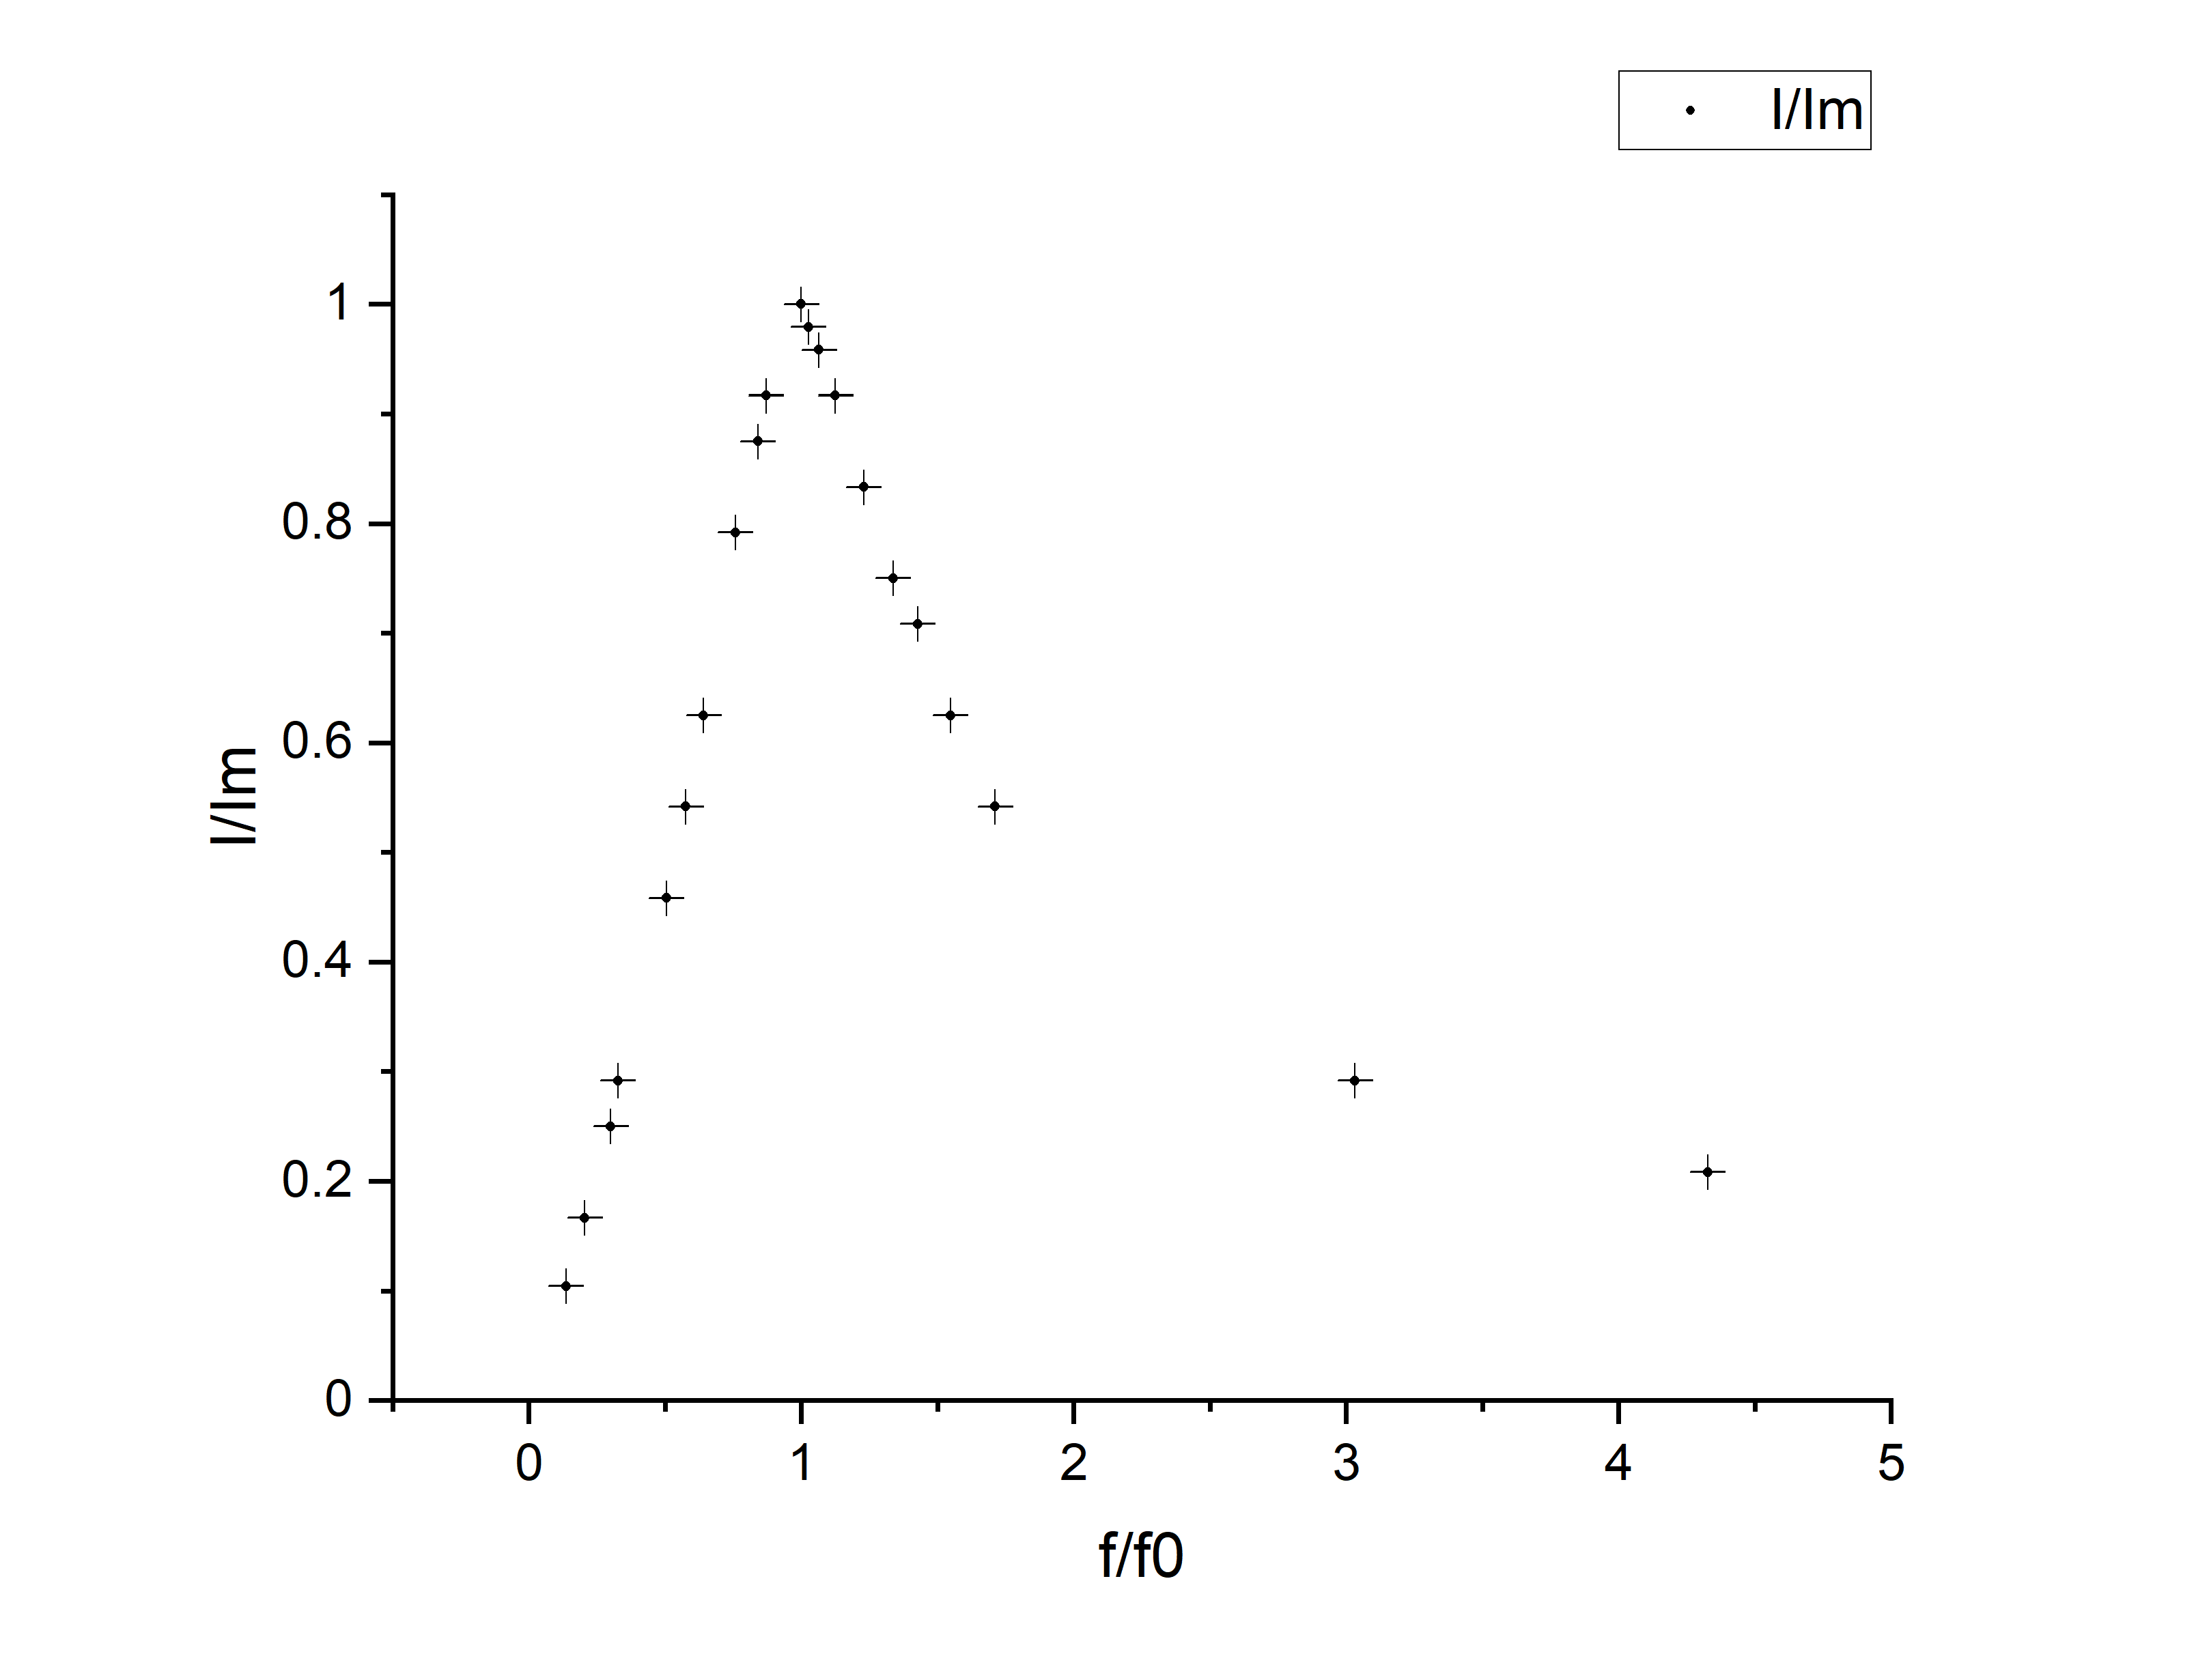
\includegraphics[scale=0.4]{6.jpg}
    \caption{I/Im vs. f/f0 plot with uncertainty.}
    \label{I/Im vs. f/f0 plot with uncertainty.}
\end{figure}
\begin{figure}[H]
    \centering
    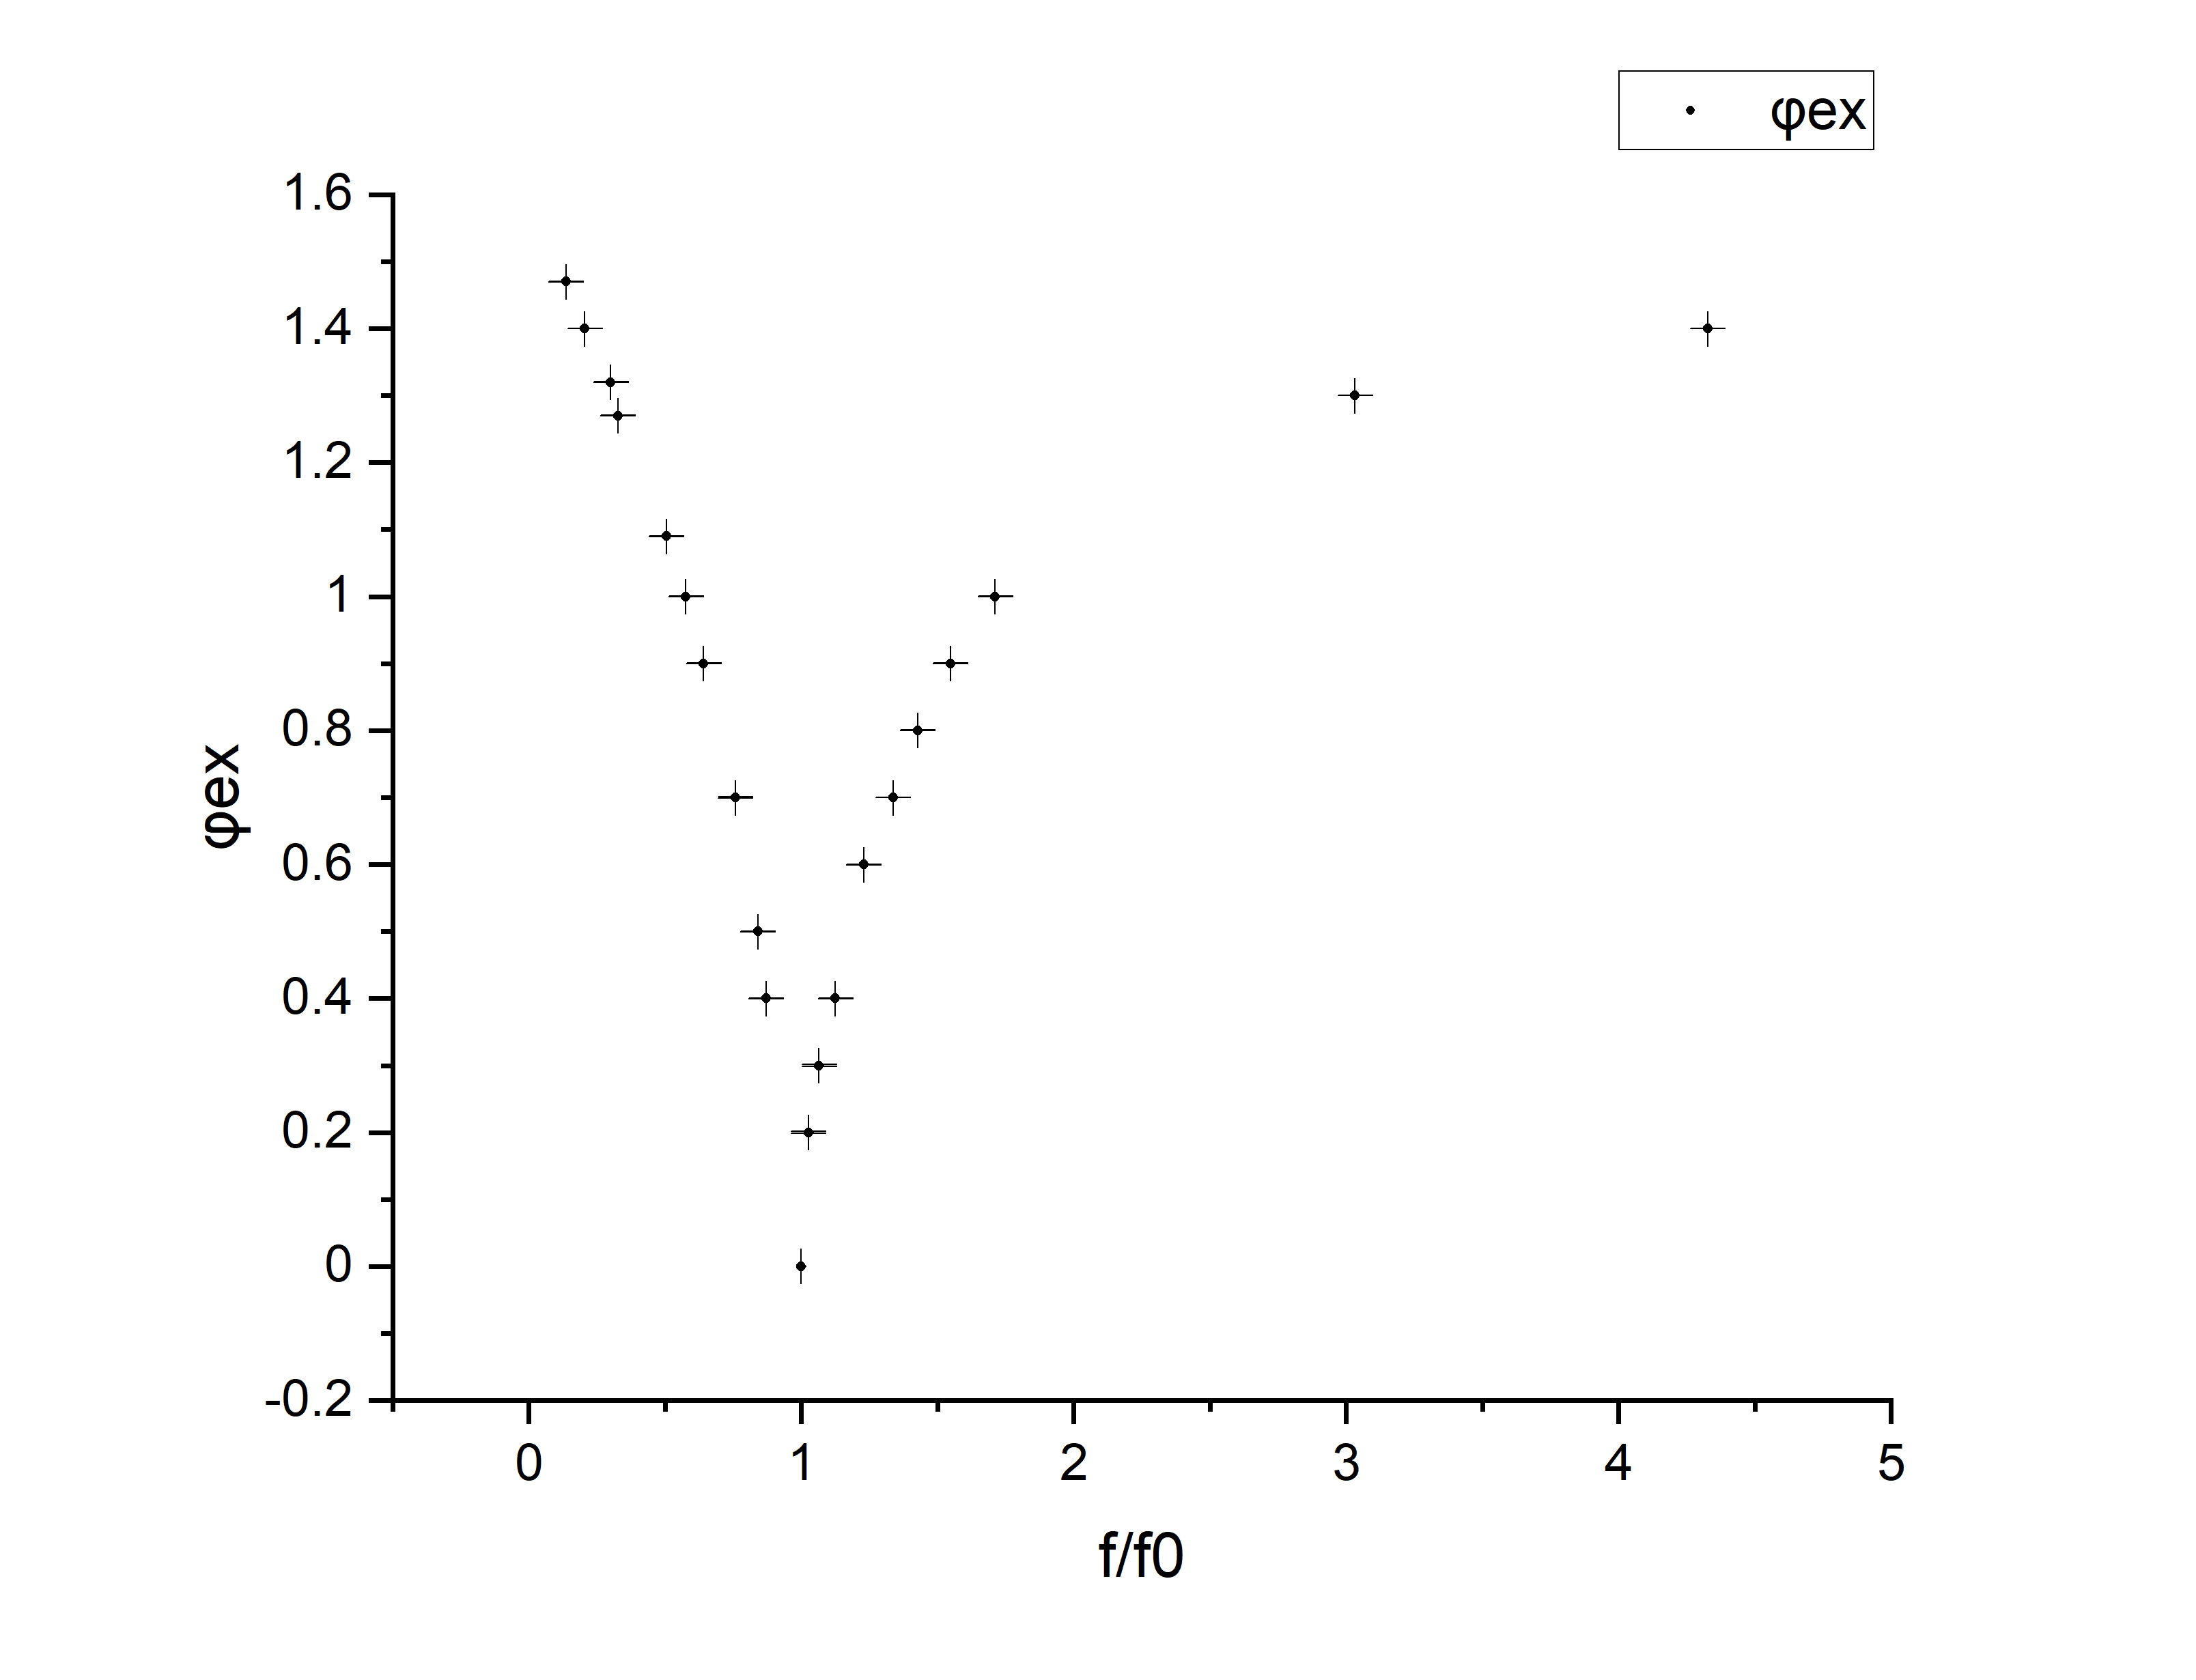
\includegraphics[scale=0.4]{4.jpg}
    \caption{$\phi$th vs. f/f0 plot with uncertainty.}
    \label{th vs. f/f0 plot with uncertainty.}
\end{figure}
\begin{figure}[H]
    \centering
    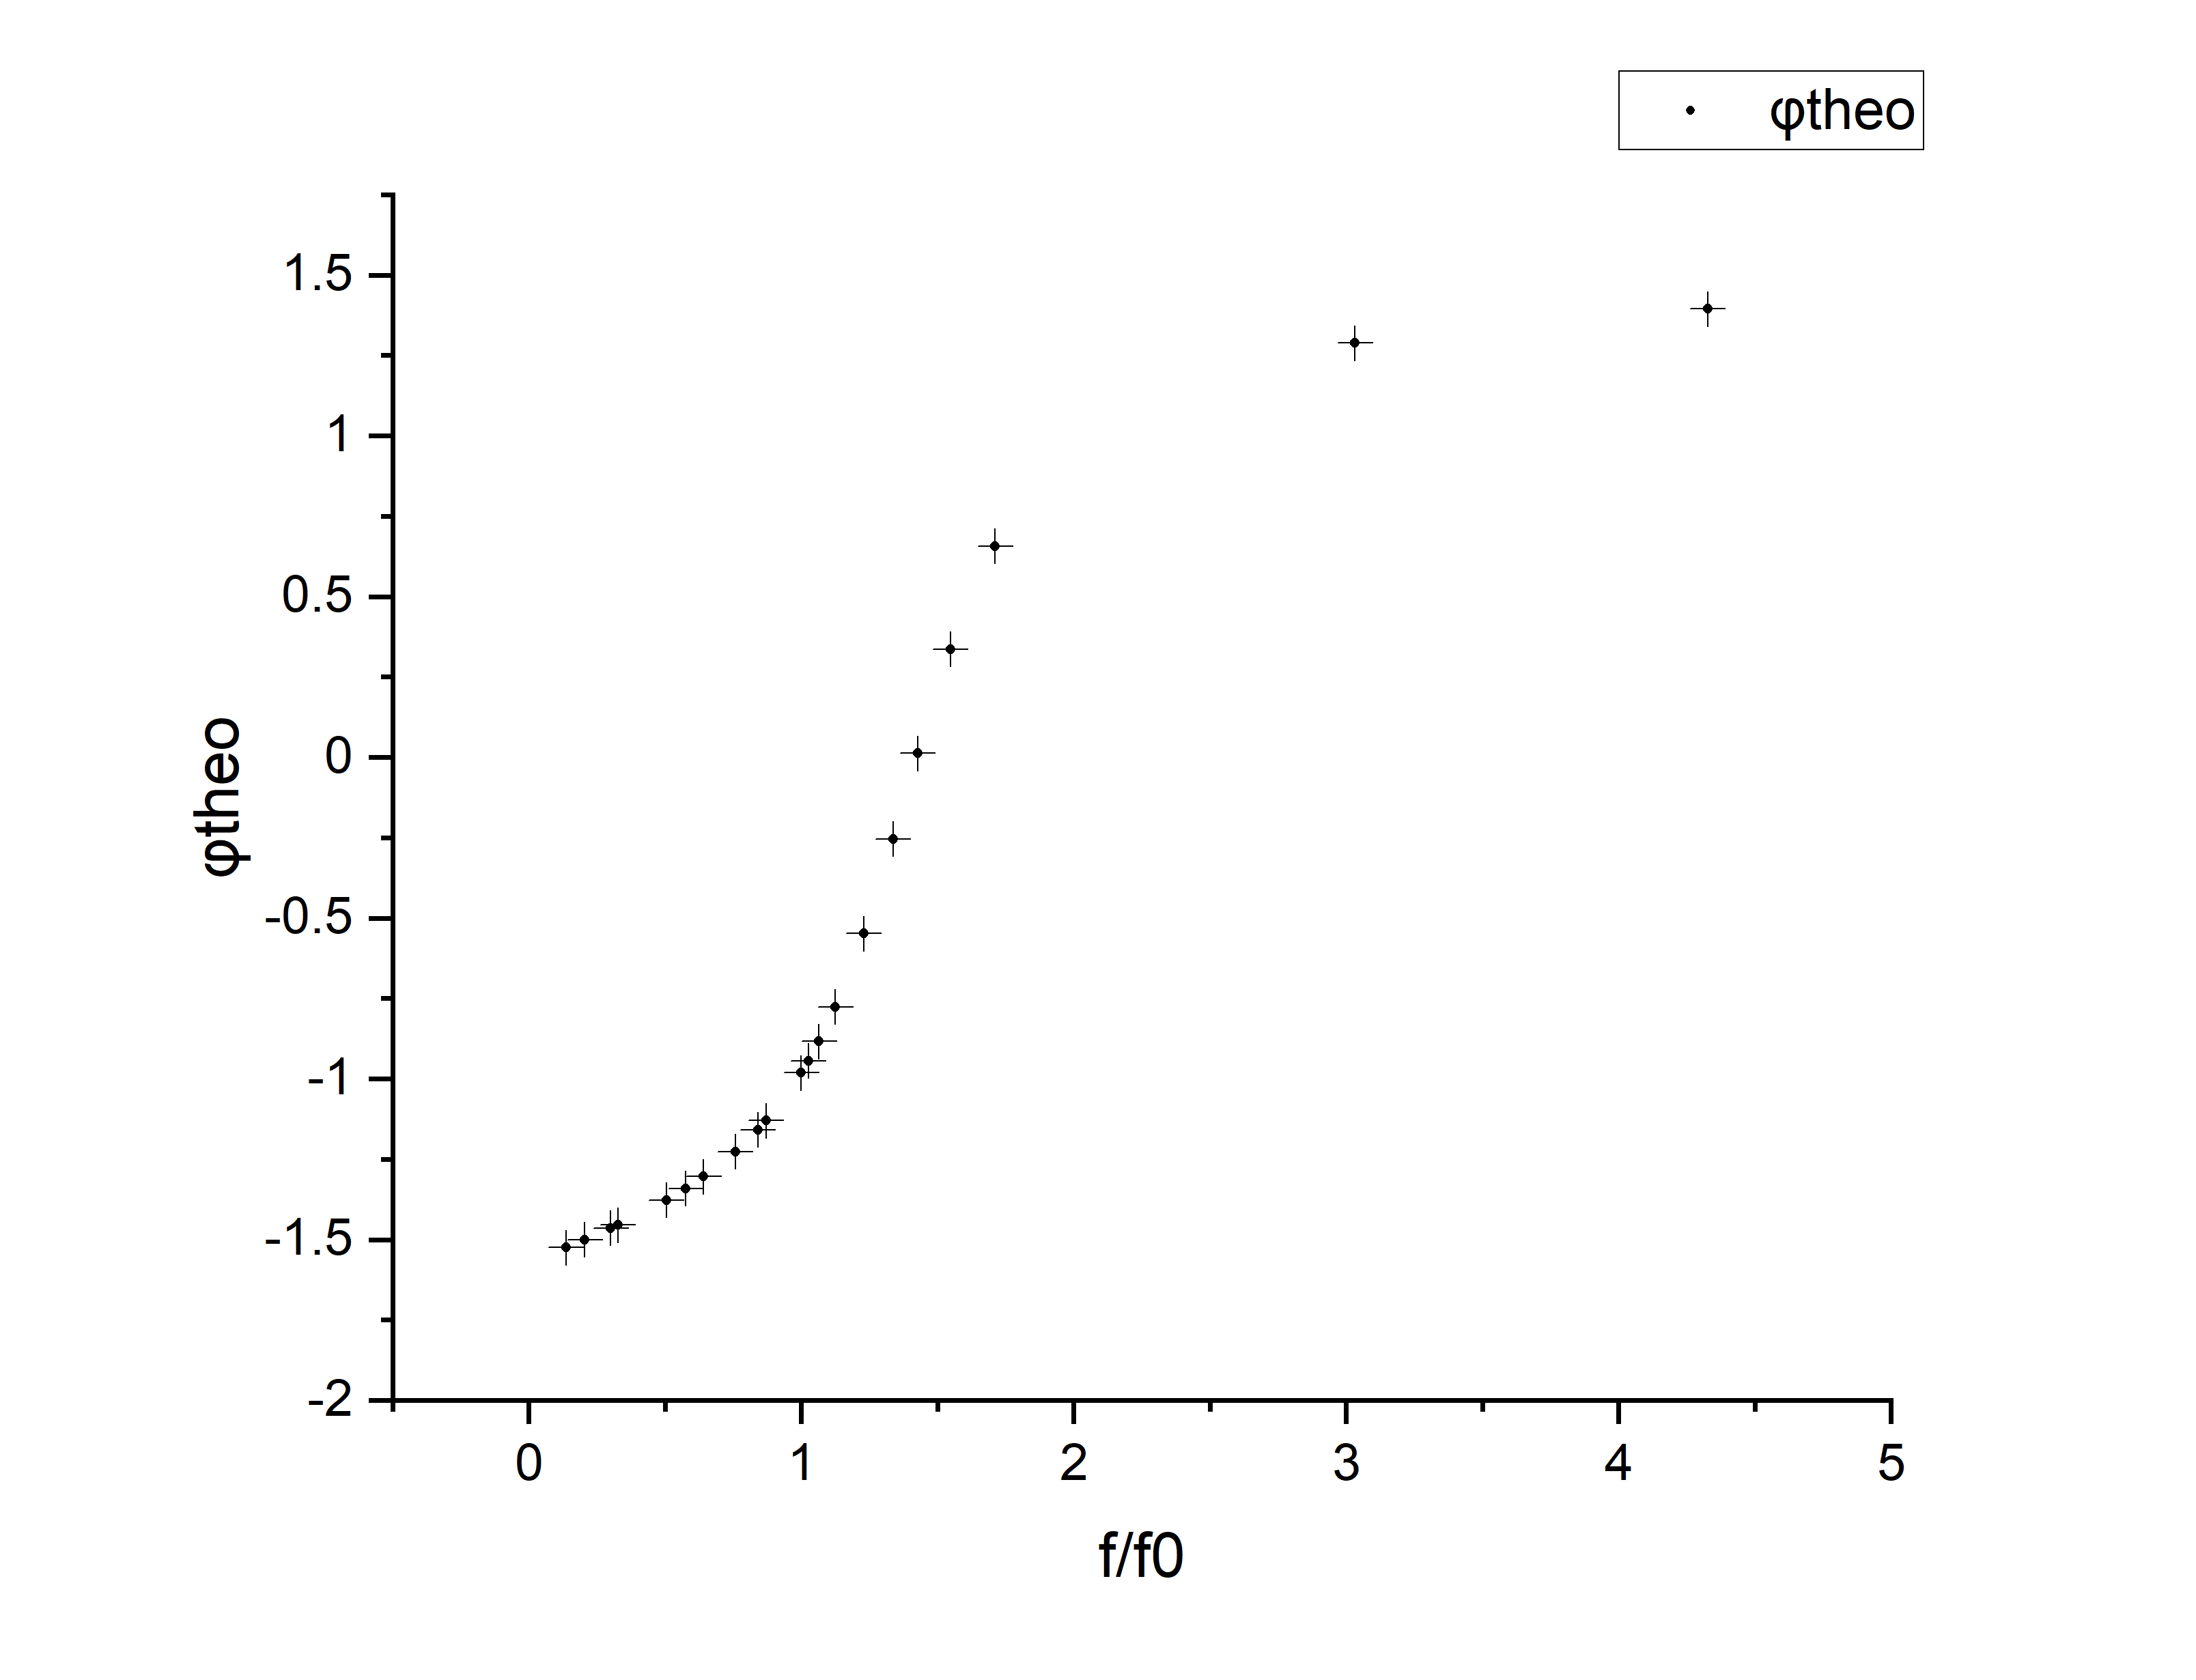
\includegraphics[scale=0.4]{5.jpg}
    \caption{$\phi$ex vs. f/f0 plot with uncertainty.}
    \label{ex vs. f/f0 plot with uncertainty.}
\end{figure}


\section{Conclusions}
\qquad As a whole, we get three sets of experimental and theoretical value of time constant $\tau$. For three sets of data, we each get the relative error to be $99.1\%,~3.8\%,~38.1\%$. And get three graphs of different damping regimes which basically conform to the theoretical graph. In the reasonance part, the experimental and theoretical value of resonance frequency f0 is found and they're calculated to have $-29.7\%$ reltiave error. Also, the theoretical and experimental value of quality factor Q is discussed and get the relative error $-28.0\%$. The relationship of f/f0 with I/Im and $\phi_{ex}$ and $\phi_{th}$ are studied by graph.\par
However, we can find that the outcome is not that ideal, we can see most of the relative error is very large, so that the outcome is not that convincing and it seems that the experiment isn't that successful to prove the theroy. However, I first notice that the relative error for the second set of time constant is very small while the first one is the largest. And I consider it to be somehow related to C and L since the first theoretical value is determined by C and the second one is determined by L.\par
And in the quality factor part, I then try another approach, which is $Q=\omega_0 L/R$ and get Q to be roughly 1.46. And the relative error than becomes $2.1\%$, which justifies the idea that the value of C somehow get wrong. Adjusting C according to the first experimental value to be around 0.467$\mu f$ and we get the other uncertainty to be $3.8\%,~2.3\%,-4.6\%,2.7\%$, which are rather small. According to the experiment procedure, the problem is mainly caused by the measurement device.\par
From this point of view, we can basically say that although there're some problems, the experiment illustrates the theories well. And for the suggestion, I think that many of the equipments should be renewed since the uncertainty is too large.




\section{References}
1.Bell, David A. Fundamentals of Electric Circuits. Oxford Univ. Press, 2009.\\
2.Qin Tian, Feng Yaming, Gu Yichen, Mateusz Krzyzosiak, Physics Laboratory VP241 Exercise 5 RC, RL, and RLC Circuits.\\
3.Young, Hugh D., et al. University Physics. Pearson, 2014. 


\end{document} 